\chapter{Metodologia}\label{metodologia}

Neste capítulo pretende-se apresentar toda a metodologia utilizada durante a
pesquisa realizada, podendo ser um norte para a reprodução da mesma em trabalhos
futuros. Inicialmente, a questão de pesquisa a ser respodida com este trabalho era a
seguinte:

\begin{center}
  \textit{Como podemos monitorar e acompanhar métricas de ameaças de
    vulnerabilidade de código fonte dentro do ciclo de desenvolvimento de
    software?
}
\end{center}

Na primeira parte do trabalho foram levantadas algumas hipóteses com relação ao
monitoramento das métricas de ameaças de vulnerabilidades de código fonte,
levando em consideração trabalhos já realizados sobre métricas de orientação a
objetos e de tamanho, como o trabalho de \citeonline{meirelles2013}. As hipóteses
foram as seguintes:

\begin{itemize}
  \item \textit{H1}: As métricas de ameaças de vulnerabilidade de código fonte
  podem ser observadas de maneira similar às métricas de \textit{design} de código
  fonte.

  \item \textit{H2}: A média dos valores das métricas de ameaças de vulnerabilidade de
  código fonte, geralmente, não é representativa para o acompanhamento das mesmas.

\end{itemize}

Ao final da primeira parte da pesquisa foram respondidas as hipóteses levantadas
inicialmente. Através da análise das métricas de ameaças de vulnerabilidade de
código fonte extraídas do projeto \textit{Linux Kernel} pode-se perceber que boa
parte dos valores das métricas eram nulos (zero), o que faz sentido, já que
espera-se que não exista ameaças de vulnerabilidades em todos os módulos do
projeto. Dessa forma, as métricas de ameaças de vulnerabilidade não se
assemelham com métricas de \textit{design} de código, pois as métricas de
\textit{design} de código não costumam ter valoração nula na maioria dos casos
devido a sua própria natureza, logo, ambas não podem ser observadas de maneira
similar, negando a hipótese \textit{H1}. Além disso, em um conjunto de valores
em que a grande maioria é zero não se pode considerar a média dos mesmos
representativa, o que nega a hipótese \textit{H2}.

Foi realizado um estudo qualitativo das métricas em questão, foram analisados
outros dez projetos, que podem ser vistos no apêndice
\ref{anex:analise_qualitativa}. Após uma análise mais detalhada dos valores das
métricas dos projetos chegou-se a um subconjunto mais frequente das mesmas em
projetos de software livre, sendo elas:

\begin{itemize}\label{principais_vuln}
  \item Referência a ponteiros nulos (CWE 476)
  \item Variáveis não inicializadas (CWE 457)
  \item Vazamento de memória (CWE 401)
\end{itemize}

Esses cenários de vulnerabilidades identificados na primeira etapa da pesquisa
serviram de insumo para a continuação da mesma, que será apresentada no decorrer
deste capítulo, para saber mais sobre as CWEs (\textit{Common Weaknesses
Enumaration}) leia a Seção \ref{cwe}.

Apesar de obter algumas respostas nesse início de pesquisa outras questões
foram levantadas, direcionando a pesquisa para a definição de modelos de
predição explicados a seguir.




\section{Trabalhos Relacionados}\label{metodologia:trabalhosrelacionados}

Durante a pesquisa realizada encontrou-se alguns trabalhos voltados para a
avaliação de ferramentas de análise estática de ameaças de vulnerabilidade de
código, como em \citeonline{comparision_bug_finding:2004}, não levando em conta
o ciclo de desenvolvimento de software, mas apenas o desempenho das ferramentas.

Em \citeonline{fault_detection:2006}, foi analisada a efetividade de ferramentas
de análise estática desse tipo, tendo como parâmetro os testes e o número de
falhas reportadas pelos clientes. Conclui-se que ferramentas de análise estática
são efetivas para encontrar defeitos a nível de código, entretanto, não é
apresentada uma solução para como monitorar os mesmos.

No trabalho realizado pelo \textit{National Institute of Standards and
Technology} (NIST) \cite{nist_effect_static_analysis:2007} foi feito um estudo
inicial tentando identificar se a inserção de uma ferramenta de análise estática
de vulnerabilidades de código fonte dentro do ciclo de desenvolvimento de um
software aumenta a segurança do mesmo. E a conclusão desse trabalho foi que não
necessariamente a utilização dessas ferramentas melhora a segurança do
software. A definição de modelos para o monitoramento dessas ameaças de
vulnerabilidade de código fonte não foi abordado nesse trabalho.

Entretanto, não se encontrou um trabalho que tentasse definir algum modelo
estatístico para monitorar e controlar métricas de ameaças de vulnerabilidade de
código fonte dentro do ciclo de desenvolvimento de um software.




\section{Planejamento da Pesquisa}\label{metodologia:planejamentopesquisa}

Com o objetivo de definir modelos de predição para as métricas de ameaças de
vulnerabilidade de código fonte aqui trabalhadas, a questão de pesquisa
redefinida é:

\begin{center}
  \textit{Existe uma função matemática que possibilite a definição de um modelo de
  predição para o monitoramento de métricas de ameaças de vulnerabilidades de
  código fonte?}
\end{center}

Tendo essa questão de pesquisa em mente o objetivo deste trabalho é encontrar
uma função matemática que viabilize o monitoramento e acompanhamento dessa classe de
métricas. E para encontrar esse meio de realizar esse monitoramente e
acompanhamento foram levantadas seguintes as hipóteses:

\begin{itemize}\label{hipoteses2}
  \item \textit{H3}: Os valores das métricas de ameaças de vulnerabilidade de
    código fonte se comportam como distribuições estatísticas de cauda longa, e
    não distribuições estatísticas normalizáveis.

  \item \textit{H4}: A definição de um modelo baseado em uma função polinomial
   simples possibilita o monitoramento e acompanhamento das métricas de ameaças
   de vulnerabilidade de código fonte.
\end{itemize}

Através de uma análise exploratória dos dados espera-se responder a hipótese
\textit{H3}, onde será possível ter uma visão geral dos dados. E através da
definição e validação de modelos estatísticos será possível responder a hipótese
\textit{H4}.

Com o intuito de responder as hipóteses levantas, foi definido um fluxo de
atividades para sistematizar esta pesquisa. A Figura \ref{fig:processo}
apresentada a seguir, ilustra o processo com o fluxo de atividades que foram
desenvolvidas, a fim de uma melhor compreensão do trabalho realizado.

\begin{figure}[h]
  \centering
  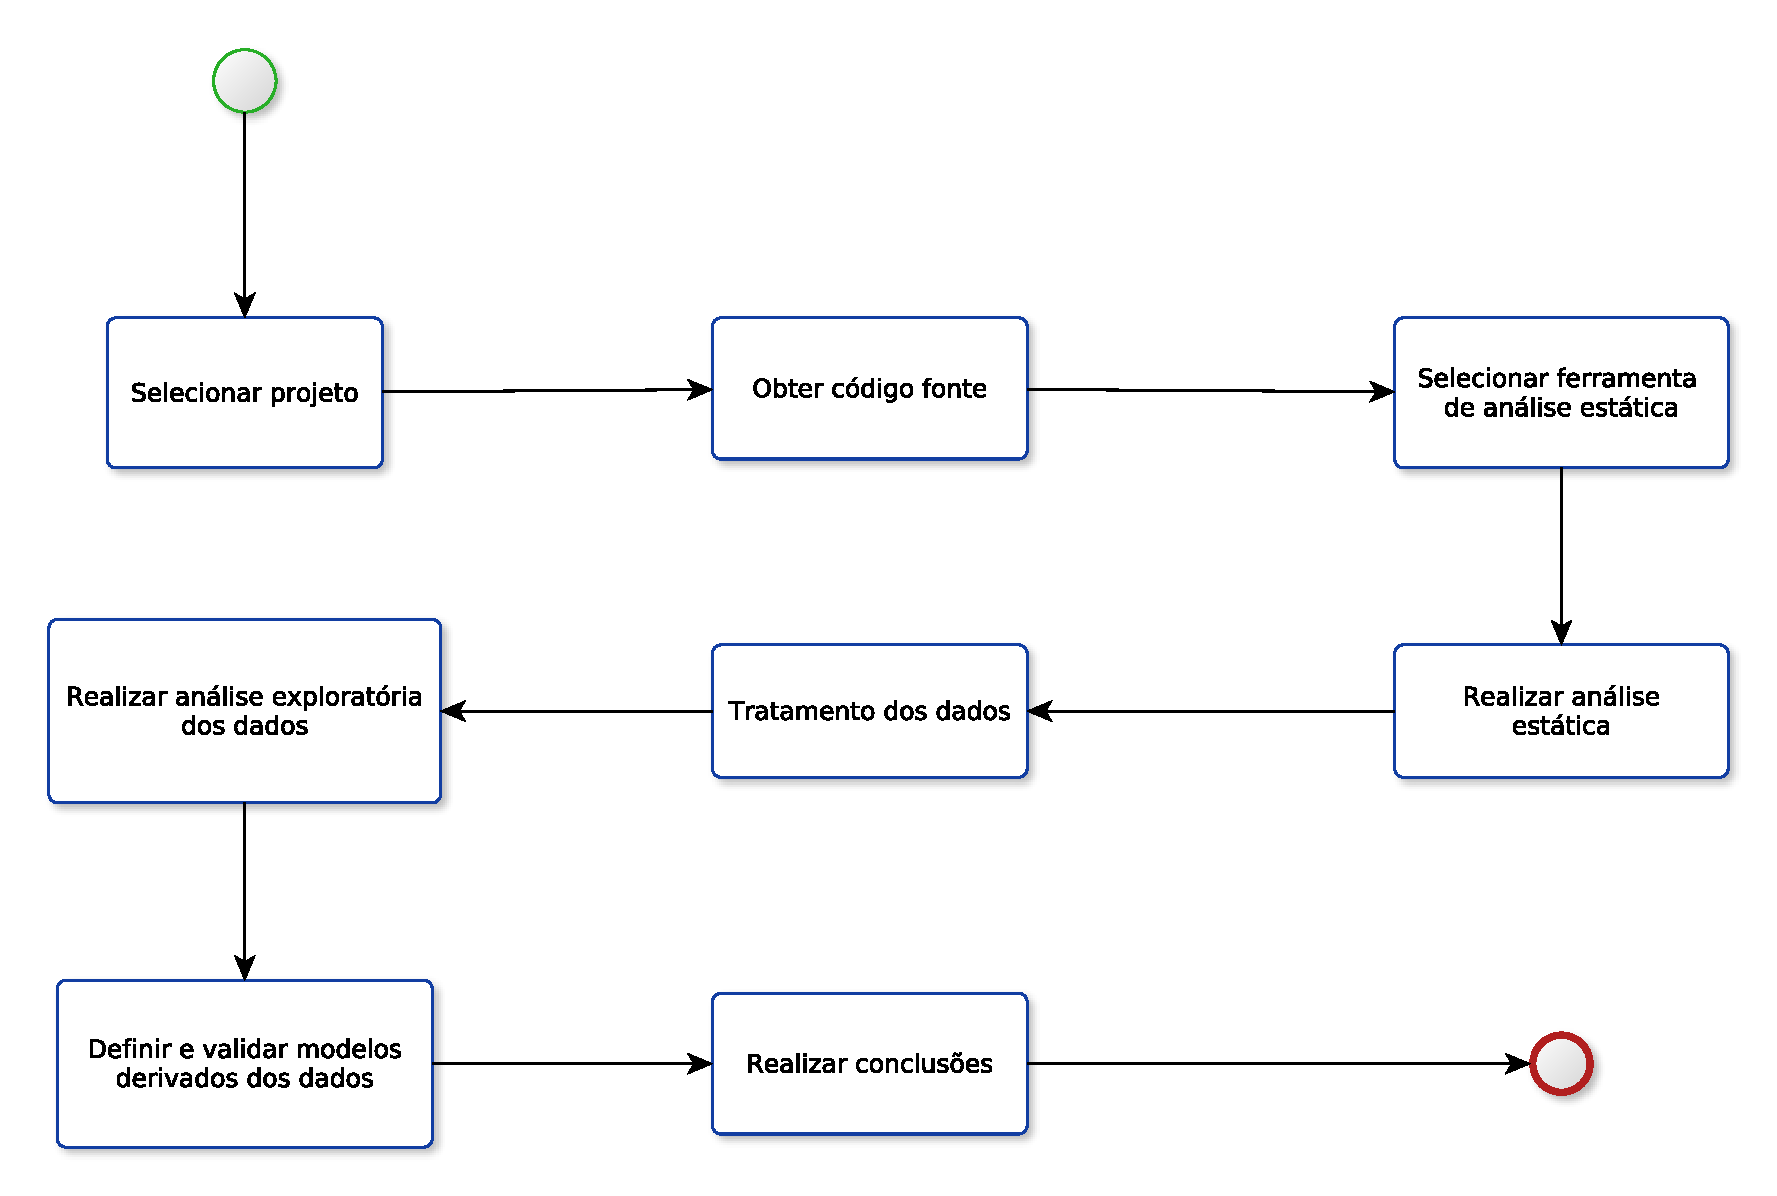
\includegraphics[width=0.9\textwidth]
      {figuras/metodologia_processo.eps}
  \caption{Processo contendo atividades executadas durante a pesquisa}
  \label{fig:processo}
\end{figure}

Detalhamento das atividades apresentadas na Figura \ref{fig:processo}:

\begin{enumerate}
  \item \textbf{Selecionar projeto}: Selecionar projeto de software livre
  representativo no contexto de segurança, para que possa ser feita a análise
  sobre o mesmo. O projeto deve ser um projeto já consolidado e com várias
  versões para que possa ser feita uma análise através do tempo.

  \item \textbf{Obter código fonte}: Obter código fonte das versões disponíveis
  do projeto selecionado, para que possa ser realizada a análise estática. A
  obtenção do código fonte deve ser feita de forma automatizada.

  \item \textbf{Selecionar ferramenta de análise estática}: Analisando os pontos
  fortes e fracos das ferramentas disponíveis, selecionar a ferramenta que
  melhor se adeque ao contexto em questão.

  \item \textbf{Realizar análise estática}: Realizar a análise estática sobre o
  código fonte obtido com a ferramenta selecionado de maneira automatizada.

  \item \textbf{Tratamento dos dados}: Ajustar o formato de saída da ferramenta
  utilizada para um arquivo CSV (\textit{Common Separated Values}) se a
  ferramenta não prover, além de tratar os dados descartando o que não for
  preciso e compondo os dados para gerar novos dados se necessário. Também deve
  ser feito de forma automatizada.

  \item \textbf{Realizar análise exploratória dos dados}: Utilizando uma
  ferramenta estatística, explorar os dados a fim de entender o comportamento do
  mesmo, para que facilite a dedução de um modelo próximo do real.

  \item \textbf{Definir e validar modelos derivados dos dados}: Encontrar
  modelos estatísticos (funções matemáticas) para monitoramento, acompanhamento e
  previsão das métricas de ameaças de vulnerabilidade de código fonte. Validar
  os modelos com dados cujo os quais não foram contruídos.

  \item \textbf{Realizar conclusões}: Comparar os modelos definidos e validados
  e indicar qual seria o melhor modelo para o monitoramento, acompanhamento e
  previsão das métricas em questão.
\end{enumerate}


\section{Teste das Hipóteses}\label{metodologia:testehipoteses}

O projeto selecionado para testar as hipóteses foi o \textit{Linux Kernel},
assim como o mesmo foi selecionado em \citeonline{cathedral_bazaar:1997} para se
entender o ecossistema e as práticas, inclusive de engenharia de software, pela
comunidade liderado por \textit{Linus Torvalds}. Devido o \textit{Linux Kernel}
seguir um modelo \textit{Bazaar} de desenvolvimento
\cite{cathedral_bazaar:1997}, a correção de \textit{bugs}, possíveis ameaças de
vulnerabilidade, se dá de maneira muito mais rápida, o que torna interessante a
análise dessa nova classe de métricas em um software bastante consolidado. Sendo
esse o primeiro projeto a explorar a rede de colaboração de software livre nos
moldes atuais \cite{cathedral_bazaar:1997}, tornando-se uma referência.
Partiu-se do \textit{Linux Kernel} para se estudar sobre práticas de
desenvolvimento de software e a própria engenharia de software, e agora será
dado o primeiro passo com relação a definição de um modelo estatístico que
auxilie no monitoramento de métricas de ameaças de vulnerabilidade de código
fonte.

\begin{description}

\item[Obtenção do código fonte]

O código fonte do projeto \textit{Linux Kernel} foi obtido no espelho
(\textit{mirror}) do Github\footnote{\url{https://github.com/torvalds/linux}}
do repositório oficial Git do
projeto\footnote{\url{https://git.kernel.org/cgit/}}.  Fez-se uma cópia local
do repositório e foram utilizados alguns comandos \textit{bash} (via terminal)
para que a obtenção do código de todas as \textit{tags} disponíveis fosse feita
de uma única vez. Nesse repositório não havia as \textit{tags} de todas as
versões, pois o projeto passou a utilizar o Git\footnote{Ferramenta de controle
de versão descentralizado} apenas a partir da versão 2.6.11, entretanto, foi
possível obter o código de 391 \textit{tags} (da versão 2.6.11 até 3.9, contando
com todas as \textit{releases candidates} ou \textit{releases} intermediárias),
sendo considerado um número representativo e suficiente para a realização do
estudo.

\item[Seleção da ferramenta de análise estática]

A ferramenta de análise estática de código fonte selecionada para a realização
deste estudo foi o
\textit{Cppcheck}\footnote{\url{http://cppcheck.sourceforge.net/}}.  A parte
inicial da pesquisa se deu com a ferramenta \textit{Clang Static
Analyzer}\footnote{\url{http://clang-analyzer.llvm.org/}}(um submódulo do
compilador \textit{Clang}), esta ferramenta é bastante robusta e consegue capturar
bem as ameaças de vulnerabilidade de código fonte que a mesma se propõe, sendo
essa uma ferramenta que está focada em si tornar uma ferramenta completa.
Entretanto, ela faz uma análise inter-procedural do código, o que necessita da
compilação do mesmo.  Infelizmente, o projeto \textit{Linux Kernel} ainda não
suporta a sua total compilação utilizando outro compilador a não ser o
GCC\footnote{\url{https://gcc.gnu.org/}}. Existe um projeto chamado
\textit{LLVMLinux
Project}\footnote{\url{http://llvm.linuxfoundation.org/index.php/Main_Page}} que
está tentando fazer com que o \textit{Linux Kernel} possa ser compilado com o
\textit{Clang}, mas esse trabalho ainda está em andamento. Logo, decidiu-se
abandonar o \textit{Clang Static Analyzer} e encontrar uma analisador estático
cujo qual não fosse necessária a compilação do código fonte, sendo esse o
\textit{Cppcheck}, que apesar de não realizar uma análise inter-procedural, ele
se propõe a não emitir uma grande quantidade de falsos positivos, chamada
ferramenta \textit{sound}, podendo ser entendido mais na Seção
\ref{sec:classificacaoferramentas}.

\item[Análise estática do código fonte]

Após a seleção da ferramenta a ser utilizada, extrair do código fonte as
ameaças de vulnerabilidade foi relativamente simples. O código fonte referente a
todas as \textit{tags} foi armazenado em um mesmo diretório, sendo o
\textit{Cppcheck} capaz de percorrer recursivamente o diretório a procura de
arquivos de código fonte C e C++ para realizar a análise, foi necessário apenas
executar a ferramenta nesse diretório. Foram feitas algumas configurações para a
geração de um arquivo de saída para cada uma das \textit{tags}. O arquivo de
saída de todas as análises realizadas estão disponíveis no
repositório.\footnote{\url{https://github.com/lucaskanashiro/linux-analysis/tree/master/data}}

\end{description}

\subsection{Descrição dos dados e Engenharia de Características}

Levando em consideração as principais ameaças de vulnerabilidades levantadas na
primeira parte da pesquisa, que podem ser vistas na lista \ref{principais_vuln},
a saída da ferramenta foi tratada a fim de filtrar por essas ameaças de
vulnerabilidades, além de criar um arquivo \textit{CSV} com esses dados. O
tratamento dos dados e geração do arquivo \textit{CSV} foram feitos através dos
scripts disponíveis no
repositório\footnote{\url{https://github.com/lucaskanashiro/linux-analysis}},
assim como o próprio arquivo \textit{CSV} gerado. A Tabela \ref{tab:csv}
apresenta a estrutura do arquivo \textit{CSV} gerado.

\begin{table}[h]
\centering
\begin{tabular}{ccccc}
\hline
\rowcolor[HTML]{EFEFEF} 
{\textbf Version} & {\textbf CWE476} & {\textbf CWE457} & {\textbf CWE401} &
{\textbf Modules} \\ \hline
linux-vXXX    & XXX          & XXX          & XXX          & XXX     \\ \hline
\end{tabular}
\caption{Estrutura do arquivo \textit{CSV} gerado.}
\label{tab:csv}
\end{table}

A coluna ``Version'' contém a versão do \textit{Linux Kernel} analisada, as
colunas ``CWE476'', ``CWE457'' e ``CWE401'' referem-se a quantidade total de cada uma
das ameaças de vulnerabilidades em toda a versão em questão, e a coluna
``Modules'' representa a quantidade total de módulos daquela versão. A seguir são
apresentados os tipos de cada um dos dados:

\begin{itemize}
  \item \textbf{Version}: Texto
  \item \textbf{CWE476}: Inteiro >= 0
  \item \textbf{CWE457}: Inteiro >= 0
  \item \textbf{CWE401}: Inteiro >= 0
  \item \textbf{Modules}: Inteiro > 0
\end{itemize}

Uma análise levando em consideração apenas esses dados não seria interessante,
já que utilizando a quantidade total absoluta de ameaças de vulnerabilidade
corre-se o risco de versões com uma maior quantidade de módulos se sobressair
em relação as outras. Pensando nisso, foi realizada uma Engenharia de
Características, onde ao final se definiu uma taxa de ameaças de
vulnerabilidades por módulo, que é facilmente calculada dividindo o total de
cada uma das ameaças de vulnerabilidade pela quantidade total de módulos. Essa
taxa claramente representa a porcentagem de vulnerabilidades por módulo se
multiplicada por 100, nesse caso a mesma deve variar entre 0 e 1. Ao final, os
dados trabalhados durante a pesquisa ficaram da forma apresentada na
Tabela \ref{tab:data_frame}.

\begin{table}[h]
\centering
%\resizebox{\textwidth}{!}
\caption{Estrutura de dados após Engenharia de Características.}
\label{tab:data_frame}
\end{table}


\subsection{Análise Exploratória dos Dados}\label{metodologia:eda}

Tendo todos os dados tratados e uma estrutura de dados bem definida, iniciou-se
a fase de análise dos dados. Utilizou-se análise exploratória dos dados,
diferente das técnicas estatísticas convencionais.

O primeiro passo foi tentar entender os dados e como os mesmos se relacionam
entre si, para isso se utilizou de uma matriz de correlação, onde é dado o
índice de correlação entre a permutação de todas as variáveis em questão. Esse
índice varia entre -1 e 1, sendo próximo de 1 diretamente relacionada e próximo de
-1 inversamente relacionada. A Tabela \ref{tab:correlacao} apresenta a matriz de
correlação do dados coletados.

\begin{table}[h]
\centering
\begin{tabular}{ccccl}
 & \cellcolor[HTML]{EFEFEF}{Modules} & \cellcolor[HTML]{EFEFEF}{tax\_CWE476} & \cellcolor[HTML]{EFEFEF}{tax\_CWE457} & \multicolumn{1}{c}{\cellcolor[HTML]{EFEFEF}{tax\_CWE401}} \\
\cellcolor[HTML]{EFEFEF}{Modules} & 1 & \multicolumn{1}{l}{} & \multicolumn{1}{l}{} &  \\
\cellcolor[HTML]{EFEFEF}{tax\_CWE476} & - 0.2263097 & 1 & \multicolumn{1}{l}{} &  \\
\cellcolor[HTML]{EFEFEF}{tax\_CWE457} & - 0.8493021 & 0.01902783 & 1 &  \\
\cellcolor[HTML]{EFEFEF}{tax\_CWE401} & - 0.513645 & - 0.1286109 & 0.5671033 & \multicolumn{1}{c}{1}
\end{tabular}
\caption{Matriz de correlação.}
\label{tab:correlacao}
\end{table}

Através da matriz de correlação pode-se extrair algumas informações. Pode-se ver
que, em geral, as taxas de ameaças de vulnerabilidades são inversamante
proporcionais a quantidade de módulos. Ou seja, quanto menor a quantidade de
módulos, provavelmente um software ainda imaturo, maior a quantidade de ameaças
de vulnerabilidade, assim como um software mais maduro tende a ter um maior
número de módulos com uma menor quantidade de ameaças de vulnerabilidade de
código fonte. As ameaças de vulnerabilidade em geral não possuem correlação, a
exceção seria entre a CWE457(variáveis não inicializadas) e a CWE401(vazamento
de memória), que segundo a matriz podem se correlacionar de maneira direta. Isso
pode ser levado em consideração tendo em vista que quando se declara uma
variável e não a utiliza, existe uma boa chance da mesma cair em esquecimento e
aquela região de memória não ser mais desalocada.

Após entender um pouco mais sobre a corelação entre os dados, foi feito um
\textit{scatterplot} (Figura \ref{fig:scatterplot}) de todas as taxas de ameaças
de vulnerabilidade pelo número de módulos para a melhor visualização dos dados.

\begin{figure}[h]
  \centering
  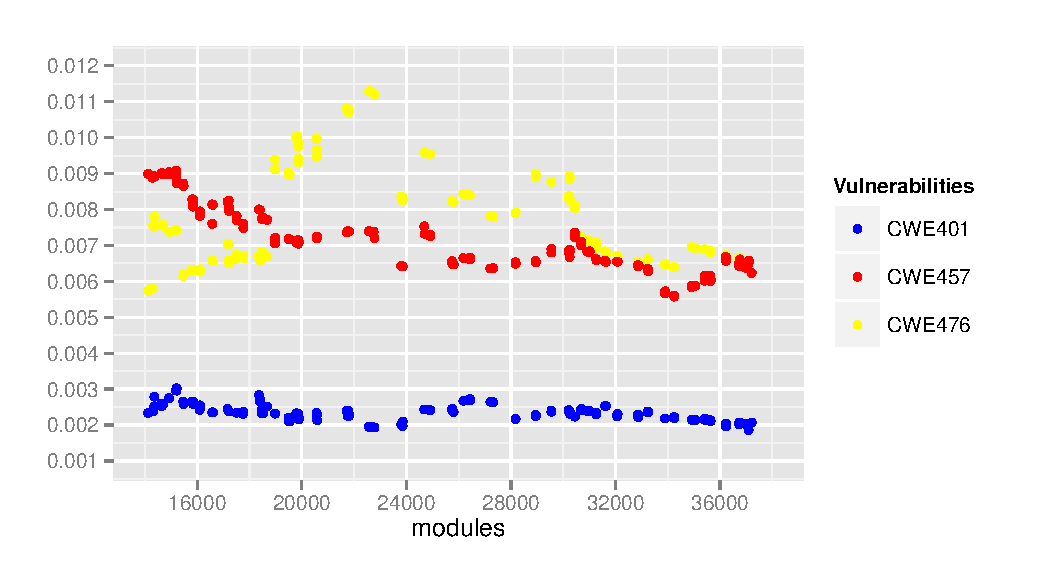
\includegraphics[width=1.0\textwidth]
      {figuras/scatterplot.eps}
      \caption{\textit{Scatterplot} das taxas de ameaças de vulnerabilidade por
      módulo pelo número total de módulos}
  \label{fig:scatterplot}
\end{figure}

As taxas, como esperado são números bem pequenos, já que o número total de
ameaças de vulnerabilidade de código fonte são bem menores do que o número total
de módulos.

Analisando o \textit{scatterplot} pode-se observar que, como foi percebido com a
análise da matriz de correlação, a taxa das ameaças de vulnerabilidade por módulo
tendem a diminuir quando se aumenta o número de módulos, provavelmente o projeto
de software está crescendo e tendo um processo de desenvolvimento mais maduro.
No início, o projeto tende a crescer e aumentar a sua complexidade, aumentando
as ameaças de vulnerabilidades, depois de certo ponto o projeto amadurece e
passa a melhorar o seu processo de desenvolvimento e \textit{design} do código
fonte, e as taxas de ameaças de vulnerabilidade tendem a cair.

Como pode-se ver, a CWE401 (vazamento de mémoria) se mantém sem muitas variações
mesmo aumentando o número de módulos. Além disso ela possui valores bem abaixo
em comparação com as outras taxas, o que nos mostra que um projeto de software
em geral, independente da sua maturidade e tamanho, não consegue sobreviver se
houver várias possíveis ocorrências de vazamento de memória, se isso ocorrer,
facilmente o software pode estourar a pilha onde é alocada memória para as
variáveis do programa. Devido a maior constância nas taxas dessa ameaça de
vulnerabilidade, não foi elaborado um modelo específico para ela, já que em
geral os valores se mantém.

Tendo isso em vista, as outras duas ameaças de vulnerabilidade de código fonte
(CWE476 e CWE457) foram estudadas separadamente a fim de ao final ter um modelo
para monitoramento e predição de cada uma.


\subsubsection{CWE476 - Referência de Ponteiros Nulos}\label{eda:cwe476}

Para analisar especificamente a ameaça de vulnerabilidade de código fonte em
questão, serão utilizados alguns gráficos para entender a taxa referente a
CWE476, para que se possa definir um modelo próximo ao real. Foram escolhidos
alguns gráficos para realizar esta análise, baseado no 4 \textit{plots}
apresentado pelo NIST (\textit{National Institute of Standards and Technology}),
como pode ser visto na Figura \ref{fig:cwe476-4-plot}.

\begin{figure}[h]
  \centering
  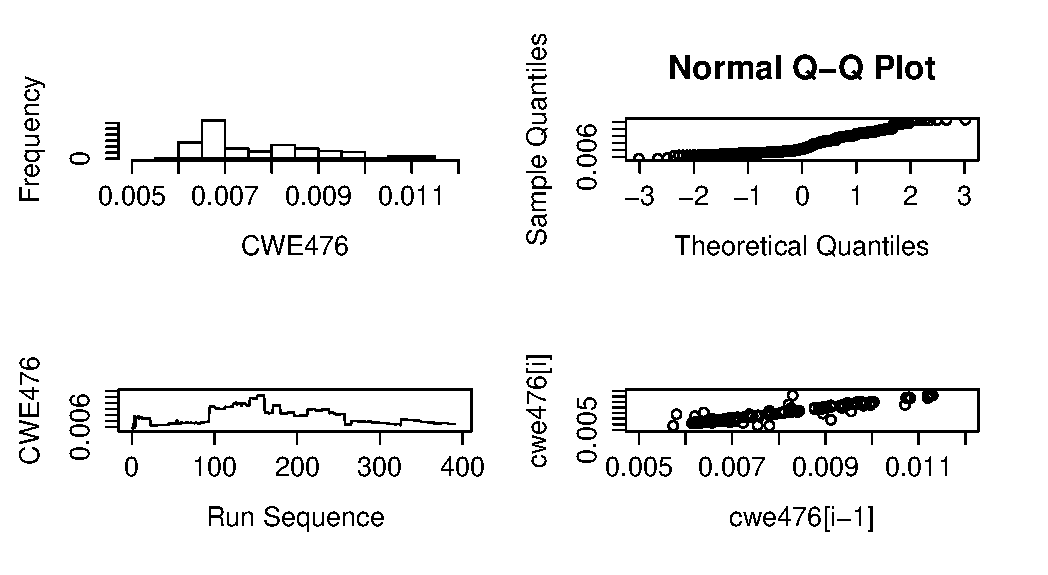
\includegraphics[width=1.0\textwidth]
      {figuras/cwe476-4-plot.eps}
      \caption{CWE476 - 4 \textit{plots}}
  \label{fig:cwe476-4-plot}
\end{figure}

Na sequência será apresentado cada um dos gráficos e feita uma discursão acerca
dos mesmos.

O primeiro gráfico apresentado na Figura \ref{fig:cwe476-4-plot} é um
histograma, onde pode-se observar a frequência da taxa desta ameaça de
vulnerabilidade. Pode ser visto com mais detalhes na Figura
\ref{fig:cwe476-hist}.

\begin{figure}[h]
  \centering
  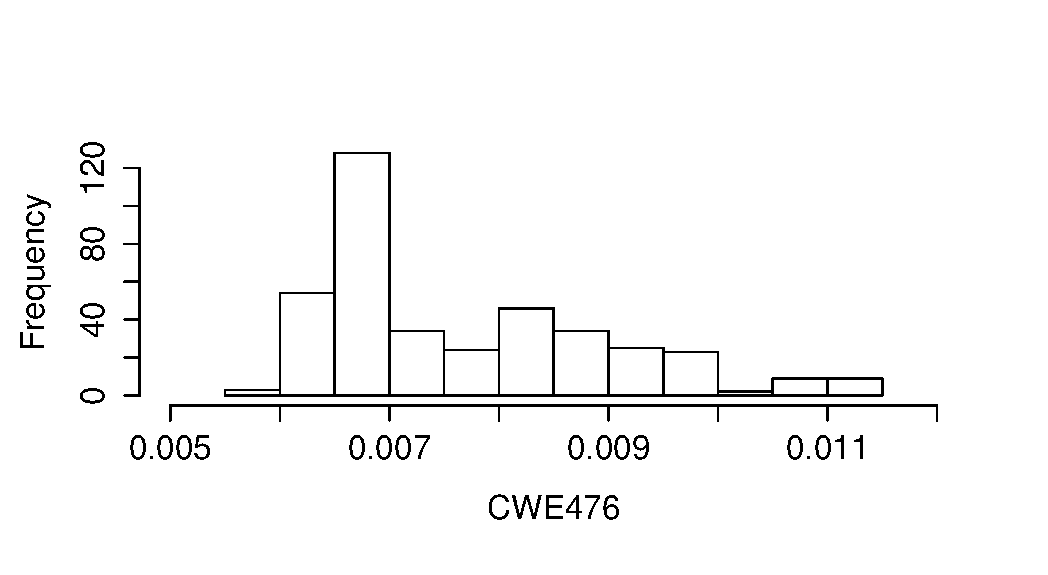
\includegraphics[width=1.0\textwidth]
      {figuras/cwe476-hist.eps}
      \caption{Histograma da taxa da CWE476}
      \label{fig:cwe476-hist}
\end{figure}

Percebe-se que a distribuição referente a esta taxa não se assemelha
a uma distribuição normal comum, já que a maior ocorrência está deslocada à
esquerda, sendo essa similar a uma distribuição de cauda longa. O maior
intervalo de ocorrência é o intervalo entre 0.0065 e 0.0070. Confirma também a
hipótese respondida na primeira parte da pesquisa, onde a média dos valores não
é representatica. O gráfico \textit{Q-Q plot} apresentado na Figura
\ref{fig:cwe476-qq-plot} vem para corroborar com o que foi dito anteriormente,
mostrando que o distribuição da taxa da CWE476 provavelmente não é uma
distribuição normal, onde a média é representativa, mas sim uma de cauda
longa.

\begin{figure}[h]
  \centering
  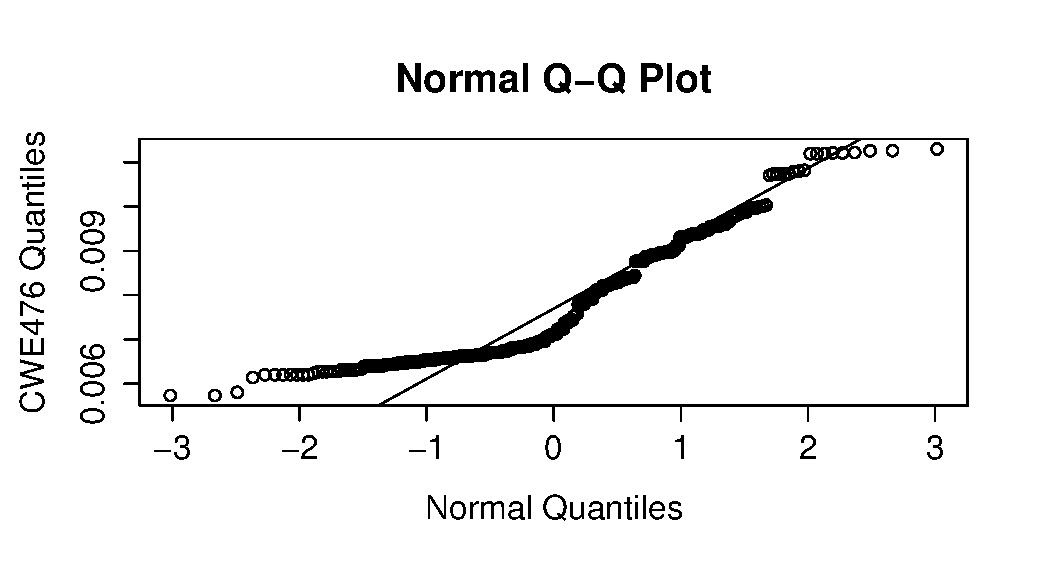
\includegraphics[width=1.0\textwidth]
      {figuras/cwe476-qq-plot.eps}
      \caption{\textit{Q-Q plot} da taxa da CWE476}
      \label{fig:cwe476-qq-plot}
\end{figure}

No \textit{Q-Q plot} são confrontados os quantis da distribuição normal e os
quantis do conjunto de dados da taxa da CWE476. Se a distribuição dos dados que
representam a taxa fosse uma distribuição normal os quantis iriam ser similares,
assim os pontos se aproximariam da reta traçada. Quanto mais próximo da reta,
mais a distribuição dos dados se assemelha a uma distribuição normal.

Na Figura \ref{fig:cwe476-run-sequence} é apresentado o gráfico de \textit{Run
Sequence}, onde o eixo x é composto de uma variável sequencial e incremental,
que começa em um e vai até o tamanho do conjunto da variável em questão (neste
caso essa variável representa as versões do \textit{Linux Kernel}), e o
eixo y é composto pelos próprios dados analisados. Com este gráfico pode-se
analisar variações locais e de escala.

\begin{figure}[h]
  \centering
  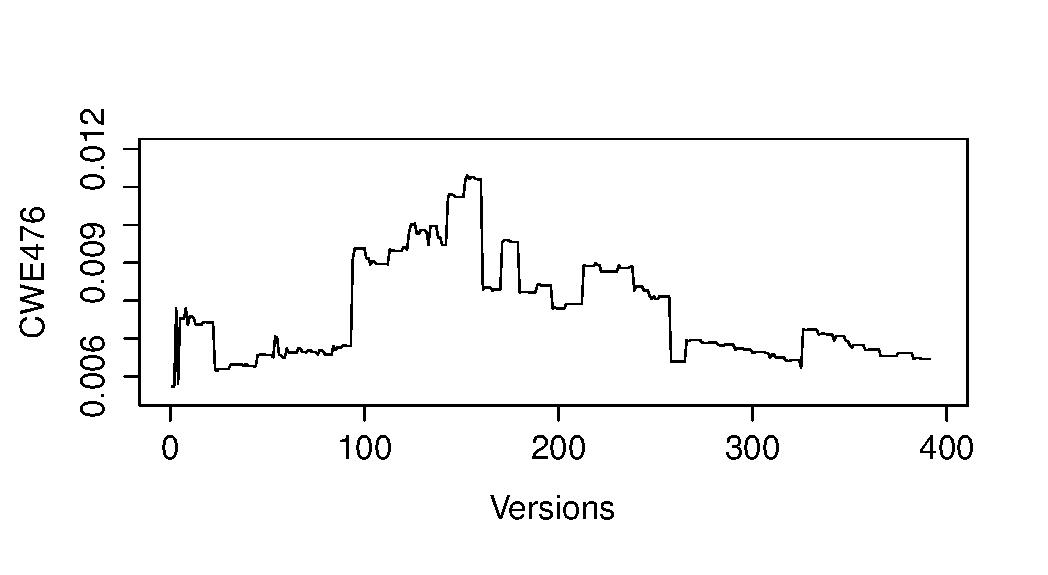
\includegraphics[width=1.0\textwidth]
      {figuras/cwe476-run-sequence.eps}
      \caption{\textit{Run Sequence} da taxa da CWE476}
      \label{fig:cwe476-run-sequence}
\end{figure}

Para um conjunto de dados que respeita a distribuição normal a variação é
praticamente constante, neste caso apresentado na Figura
\ref{fig:cwe476-run-sequence}, pode-se observar que a variação dos dados não é
constante, e possui um pico próximo a versão 150 e depois volta a diminuir a
taxa. Isso se deve a uma refatoração do código fonte do \textit{Linux Kernel}
que se iniciou após a versão 2.6.29 (versão 150) até a versão 3.0 (versão 250),
que possibilitou a redução de ameças de vulnerabilidade de código fonte.

Para encerrar a análise dos dados referentes a taxa da CWE476, é apresentado um
\textit{Lag Plot} na Figura \ref{fig:cwe476-lag-plot}. Esse gráfico nos auxilia
a identificar a aleatoriedade dos dados e a identificar um modelo que se adeque
aos mesmos. A construção se dá de maneira simples, onde no eixo y estão os
dados, e no eixo x estão os antecessores dos dados do eixo y.

\begin{figure}[h]
  \centering
  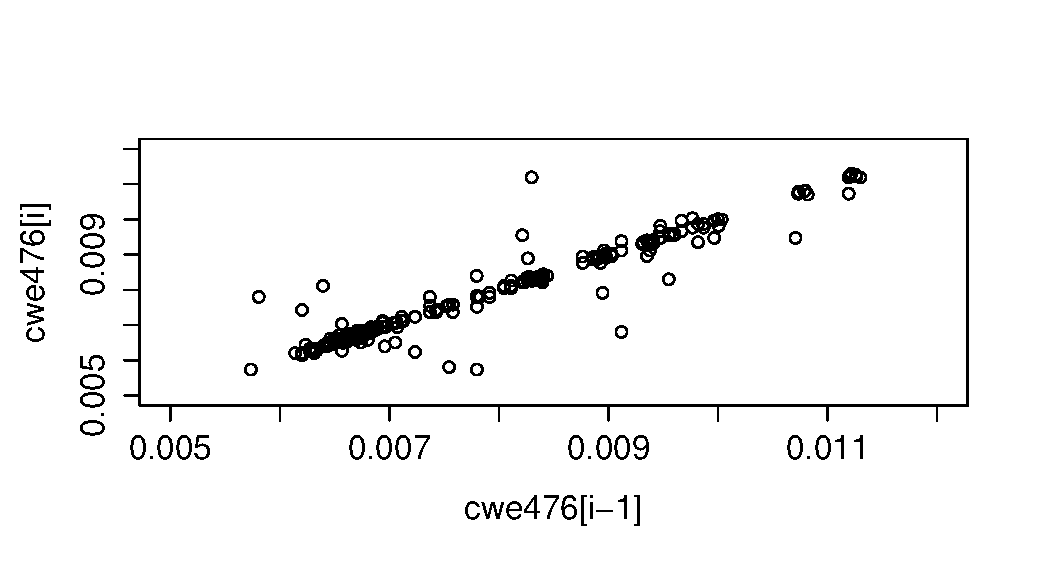
\includegraphics[width=1.0\textwidth]
      {figuras/cwe476-lag-plot.eps}
      \caption{\textit{Lag Plot} da taxa da CWE476}
      \label{fig:cwe476-lag-plot}
\end{figure}

Pela figura pode-se perceber que há uma relação linear entre os dados e os seus
antecessores, nos mostrando que este conjunto de dados não é aleatório. Sabendo
que a variação dos dados não é constante como o que acontece em um polinômio de
primeiro graus, foi realizada uma regressão para polinômios de diferentes graus
maiores do que um para tentar encontrar um que melhor se adeque, conforme será
apresentado na Seção \ref{definicaomodelos}.


\subsubsection{CWE457 - Variável não Inicializada}\label{eda:cwe457}

A abordagem utilizada para o cenário de ameaça de vulnerabilidade anterior
também será aplicada no contexto de variáveis não inicializadas. Primeiramente,
será apresentada o gráfico \textit{4 Plots}, visto na Figura
\ref{fig:cwe457-4-plot}. Em seguida serão destrinchados cada um dos referidos
gráficos,

\begin{figure}[h]
  \centering
  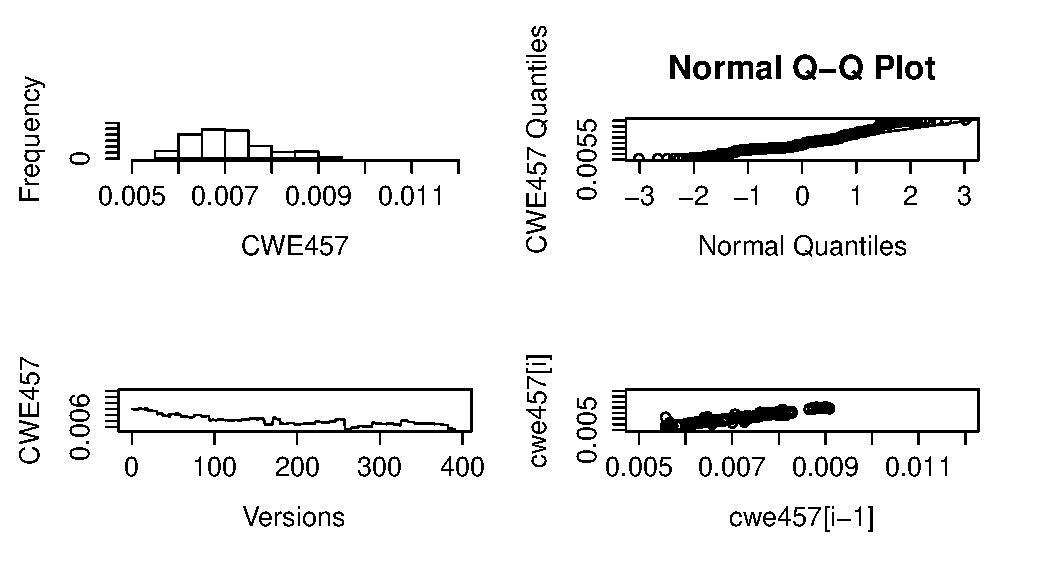
\includegraphics[width=1.0\textwidth]
      {figuras/cwe457-4-plot.eps}
      \caption{CWE457 - 4 \textit{plots}}
  \label{fig:cwe457-4-plot}
\end{figure}

Iniciando a análise pelo histograma, que pode ser visto com mais detalhes na
Figura \ref{fig:cwe457-hist}. Assim como o histograma apresentado pela taxa da
CWE476 (Figura \ref{fig:cwe476-hist}), esse aparenta respeitar uma distribuição
estatística de cauda longa ao invés de uma normal. Pode-se ver que o intervalo
de maio ocorrência é o intervalo entre 0.0065 e 0.0070, da mesma forma que o
cenário anterior.

\begin{figure}[h]
  \centering
  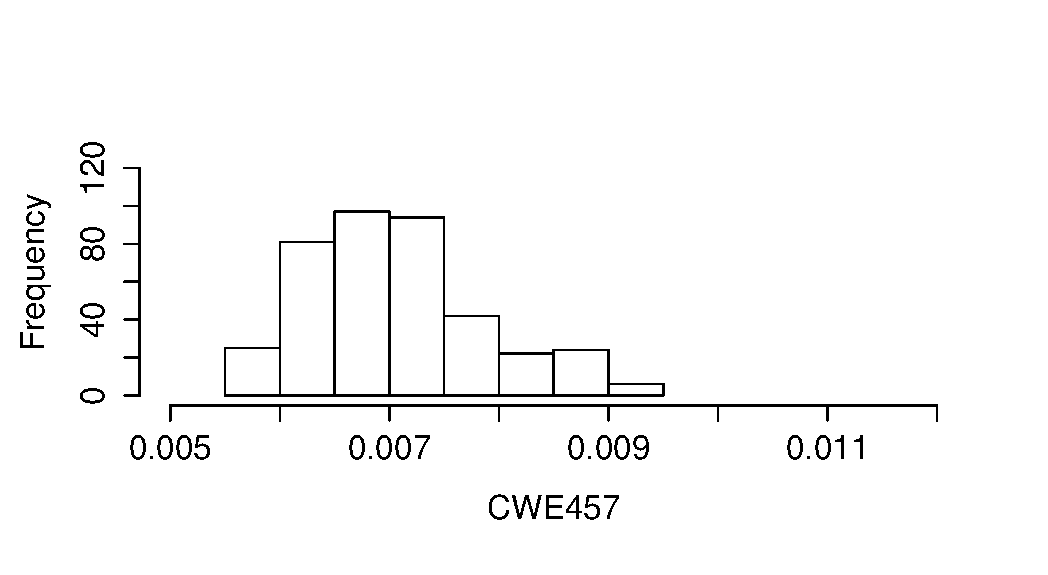
\includegraphics[width=1.0\textwidth]
      {figuras/cwe457-hist.eps}
      \caption{Histograma da taxa da CWE457}
  \label{fig:cwe457-hist}
\end{figure}

Mais uma vez é confirmanda a negação da hipótese \textit{H2}, onde a média dos
valores dessas métricas seria representativa. O gráfico \textit{Q-Q Plot} nos
auxilia a ver de maneira mais clara a não conformidade com a distribuição normal
através da Figura \ref{fig:cwe457-qq-plot}. Esse gráfico nos mostra que a
distribuição dos dados da CWE457 está mais próxima de uma normal do que a
CWE476, entretanto, pode-se dizer que a normal também não é representativa nesse
caso, pois existe uma cauda longa próxima aos maiores quantis.

\begin{figure}[h]
  \centering
  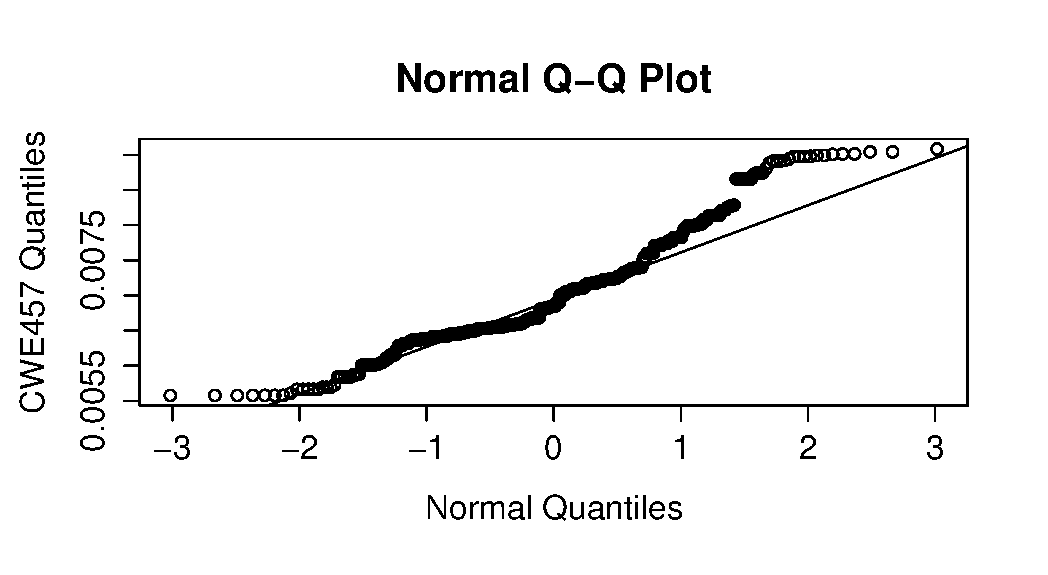
\includegraphics[width=1.0\textwidth]
      {figuras/cwe457-qq-plot.eps}
      \caption{\textit{Q-Q Plot} da taxa CWE457}
  \label{fig:cwe457-qq-plot}
\end{figure}

Analisando a Figura \ref{fig:cwe457-run-sequence} que contém um gráfico
\textit{Run Sequence}, percebe-se que a variação dos valores também não são
constantes, descartando uma regressão para um polinômio de primeiro grau.
Entretanto, não existem picos que destoam totalmente das outras variações, não
demonstrando efeito significativo da refatoção a partir da versão 150 (versão
2.6.29) com relação as variáveis não inicializadas.

\begin{figure}[h]
  \centering
  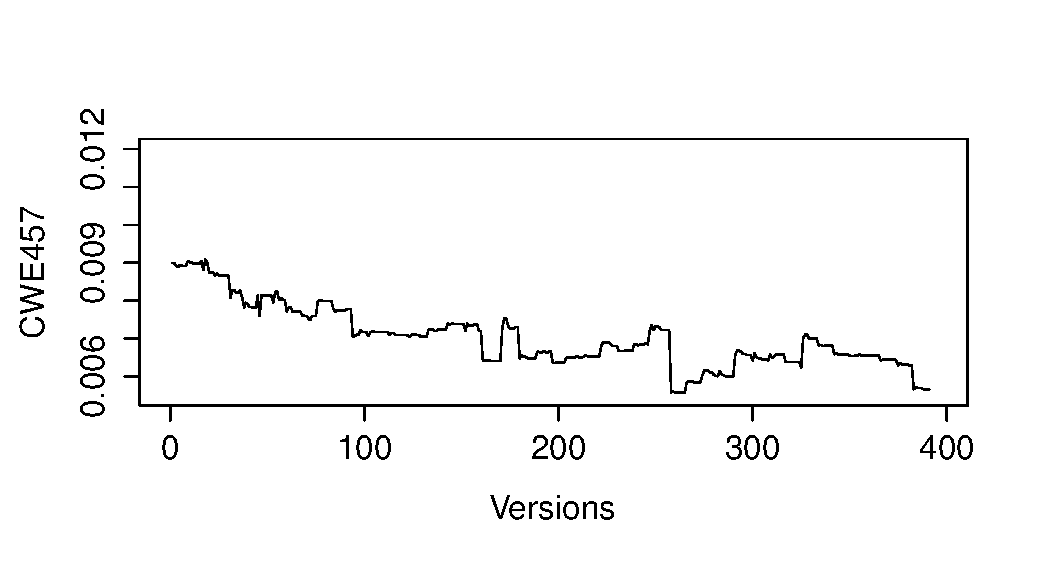
\includegraphics[width=1.0\textwidth]
      {figuras/cwe457-run-sequence.eps}
      \caption{\textit{Run Sequence} da taxa CWE457}
  \label{fig:cwe457-run-sequence}
\end{figure}

Finalizando a análise do cenário de ameaça de vulnerabilidade de variáveis não
inicializadas, é apresentado o \textit{Lag Plot} na Figura
\ref{fig:cwe457-lag-plot}. Assim como o apresentado pela CWE476 (Figura
\ref{fig:cwe476-lag-plot}), existe uma relação linear entre os dados e seus
antecessores diretos. Com isso, a decisão tomada também foi a mesma, realizar
regressões para polinômios de diferentes graus diferentes de um e tentar
confronta-los para identificar qual o melhor modelo.

\begin{figure}[h]
  \centering
  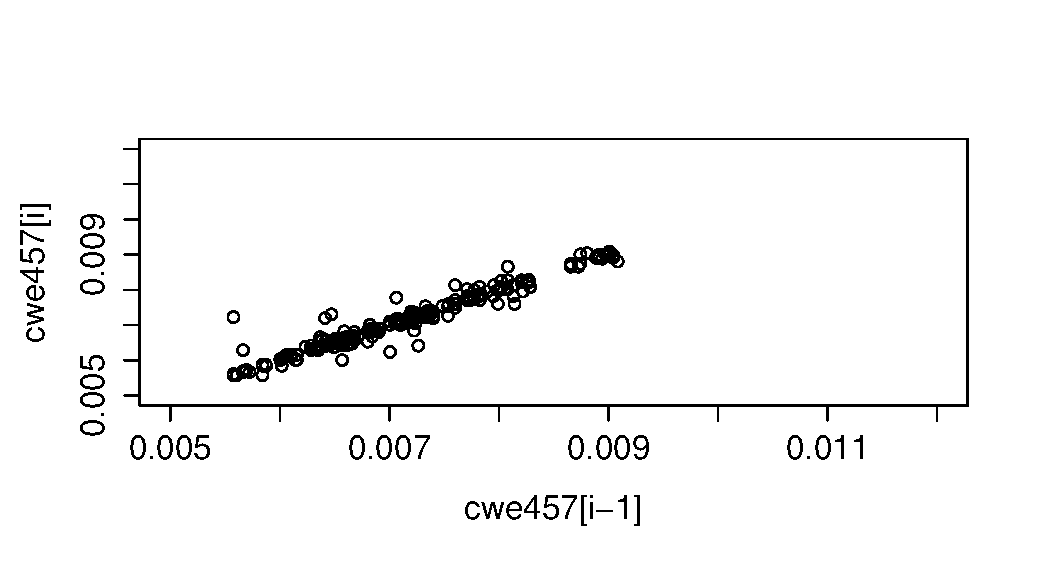
\includegraphics[width=1.0\textwidth]
      {figuras/cwe457-lag-plot.eps}
      \caption{\textit{Lag Plot} da taxa CWE457}
  \label{fig:cwe457-lag-plot}
\end{figure}


\subsubsection{Resultados Obtidos}

Após a realização do teste das hipóteses levantadas no início da pesquisa (lista
\ref{hipoteses2}) se tem insumo para chegar em algumas conclusões. A hipótese
\textit{H3} não foi negada, já que como pode-se ver nos histogramas e gráficos
\textit{Q-Q plot}, apresentados na Seção \ref{metodologia:eda}, que a distribuição das taxas
de ameaças de vulnerabilidade de código fonte trabalhadas seguem uma
distribuição estatística de cauda longa, e não uma simples distribuição normal
onde a média dos valores é representativa.  Sendo esse um ponto que já havia
sido discutido no início deste capítulo e que foi corroborado após o trabalho
realizado.

Tendo isso em vista, foram definidos modelos polinomiais para tentar testar a
hipótese \textit{H4} na Seção \ref{definicaomodelos}.
















\chapter{Definição dos Modelos de Predição}\label{definicaomodelos}

Como pode ser visto na Seção \ref{metodologia:eda}, as duas métricas de ameaças de
vulnerabilidade de código fonte trabalhadas se comportaram de maneira similar.
Mas como o intuito desta pesquisa é encontrar uma função matemática que
possibilite o monitoramento e predição de cada uma das métricas, o modelo de
ambas serão desenvolvidos separadamente, apesar de seguirem os mesmos métodos e
critérios.

As atividades realizadas para definir cada um dos modelos que serão apresentados a
seguir foram:

\begin{enumerate}
 \item Identificar e remover possíveis \textit{outliers}.
 \item Dividir o conjuto de dados em conjunto de teste e de treinamento, sendo o
  conjunto de teste um terço e o de treinamento dois terços do total.
 \item Definição de um modelo não paramétrico, que servirá de referência para a
  definição do modelo paramétrico.
 \item Definição de um modelo paramétrico, tentando se aproximar da referência
  do modelo não paramétrico.
\end{enumerate}

Foi utilizado o método de \citeonline{tukey:1977} apresentado na Seção
\ref{outliers}, para a identificação dos \textit{outliers}. Utilizou-se de um
método não paramétrico que traçasse uma curva suave baseado no
\textit{scatterplot} apenas como referência pois o mesmo não nos dá uma função
matemática como saída, apesar dos resultados do mesmo ser bastante satisfatório.
O método não paramétrico utilizado foi o \textit{LOESS} (\textit{Locally
 Weighted Regression}), como foi explicado na Seção \ref{def:models}, o mesmo tem
 como um dos seus pontos fortes a análise de uma série temporal, como a que
 estamos trabalhando, valores de métricas de uma série de versões do projeto
 \textit{Linux Kernel}.
 
 É importante salientar que pode-se representar qualquer conjunto de dados com
 um polinômio de algum grau, entretanto, para realizar predições baseado no
 modelo gerado precisa-se evitar o \textit{overfitting}, que seria o modelo se
 ajustar extremamente ao conjunto de dados e não conseguir extrapolar para novas
 entradas. Utilizando essa abordagem de utilizar um modelo não paramétrico como
 referência ajuda a evitar um possível \textit{overfitting} do modelo gerado,
 chegando a um modelo mais flexível.

Para a definição dos modelos foi utilizada a técnica de regressão polinomial,
foram construídos modelos com polinômios de diferentes graus baseado na curva
dada pelo método não paramétrico. Os modelos gerados serão comparados na Seção
\ref{comparacaomodelos}.

\section{Definição de modelo para CWE476 - Referência a Ponteiros Nulos}

Na tentativa de identificar possíveis \textit{outliers} utilizando o método de
\citeonline{tukey:1977}, foi contruído o gráfico \textit{boxplot} (Figura
\ref{fig:cwe476-boxplot}). Como pode-se ver não foram identificados
\textit{outliers} extremos, todos os pontos da distribuição dos valores da taxa
de CWE476 por módulo estão dentro dos limites determinados pelo método, que
extrapola para mais e para menos 150\% do referido interquantil.

\begin{figure}[h]
  \centering
  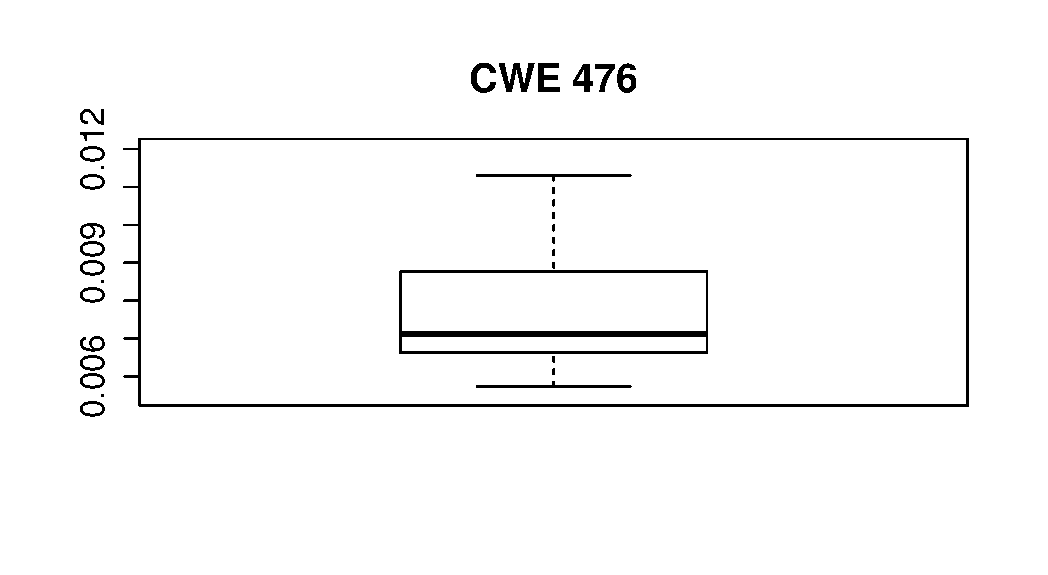
\includegraphics[width=1.0\textwidth]
      {figuras/cwe476-boxplot.eps}
      \caption{\textit{Boxplot} da taxa da CWE476 por módulo}
  \label{fig:cwe476-boxplot}
\end{figure}

Como não foram identificados possíveis \textit{outliers}, o conjunto de dados
permaneceu o mesmo, sem sofrer alterações. Com isso, passou-se a definir o
modelo não paramétrico, como resultado final se teve uma curva suavizada
bastante satisfatória, como se pode ver na Figura \ref{fig:cwe476-loess}. Sendo
a curva o resultado da predição do modelo definido sobre os dados de
treinamento. O erro residual padrão desse modelo é 0.0008044, sendo o erro
residual padrão o desvio padrão da diferença entre o valor real e o predito.

\begin{figure}[h]
  \centering
  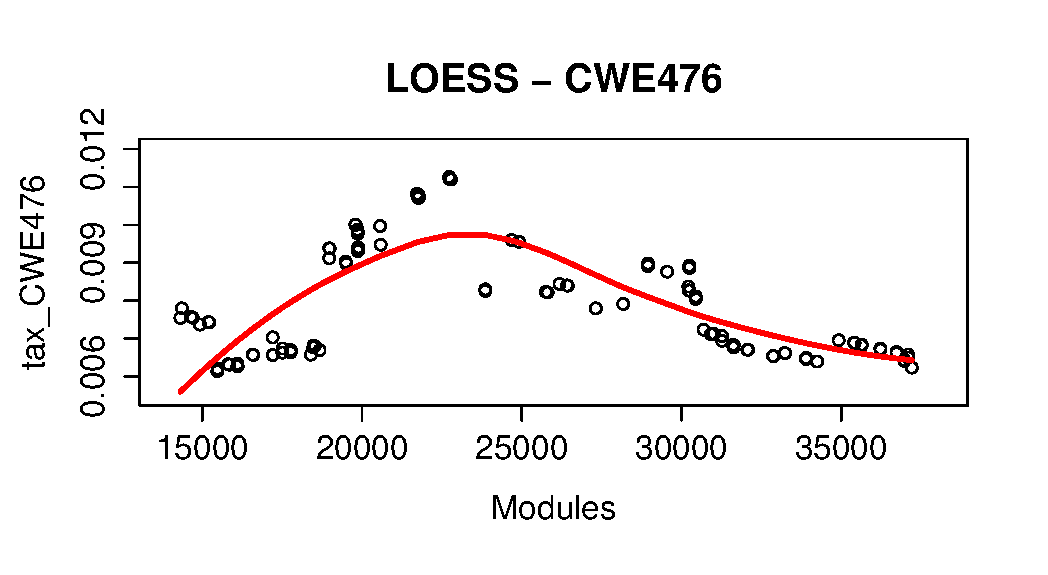
\includegraphics[width=1.0\textwidth]
      {figuras/cwe476-loess.eps}
      \caption{Curva suavizada gerada pelo método \textit{LOESS} sobre o
      conjunto de dados da taxa da CWE476 por módulo}
  \label{fig:cwe476-loess}
\end{figure}

Analisando visualmente a curva gerada pelo método não paramétrico pode-se
especular que provavelmente uma função quadrática poderia se adaptar bem ao
conjunto de dados trabalhado e se aproximar da curva apresentada. Para validação
do modelo acerca do conjunto de dados, foi desenvolvido em conjunto um modelo
cúbico visando compara-los e chegar a um modelo que se aproxime do desejado e
não seja tão custuso para calculá-lo. 

A regressão para um polinômio quadrático do conjunto de treinamento nos deu a
seguinte equação:

%\begin{tcolorbox}

 \begin{align*}
  tax\_CWE476(modules) &=& (-2.131399e^{-11}) * modules^{2} \\
                       &+& (1.057282e^{-6}) * modules \\
                       &-& 0.004237619 
 \end{align*}


%\end{tcolorbox}

Após realizada uma predição sobre o conjunto de teste, foi plotada a curva de
predição juntamento com o \textit{scatterplot} dos dados, como pode ser visto na
Figura \ref{fig:cwe476-quadratic}. O erro residual padrão para esse modelo foi
0.0009653.

\begin{figure}[h]
  \centering
  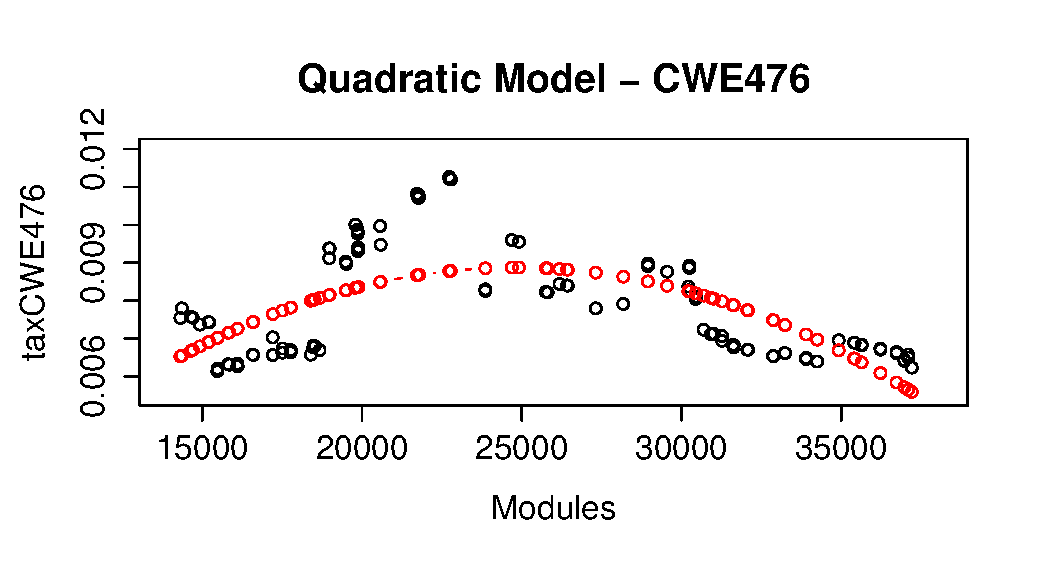
\includegraphics[width=1.0\textwidth]
      {figuras/cwe476-quadratic.eps}
      \caption{Curva de predição do modelo quadrático sobre o \textit{scatterplot}
      dos dados da CWE476}
  \label{fig:cwe476-quadratic}
\end{figure}

A regressão para um polinômio cúbico do conjunto de treinamento nos deu a
seguinte equação:

\begin{align*}
 tax\_CWE476(modules) &=& (1.911224e^{-15}) * modules^{3} \\
                      &-& (1.72028e^{-10}) * modules^{2} \\
                      &+& (4.857479e^{-6}) * modules \\
                      &-& 0.03460173
\end{align*}

Após realizada uma predição sobre o conjunto de teste, foi plotada a curva de
predição juntamento com o \textit{scatterplot} dos dados, como pode ser visto na
Figura \ref{fig:cwe476-cubic}. O erro residual padrão para esse modelo foi
0.00084.

\begin{figure}[h]
  \centering
  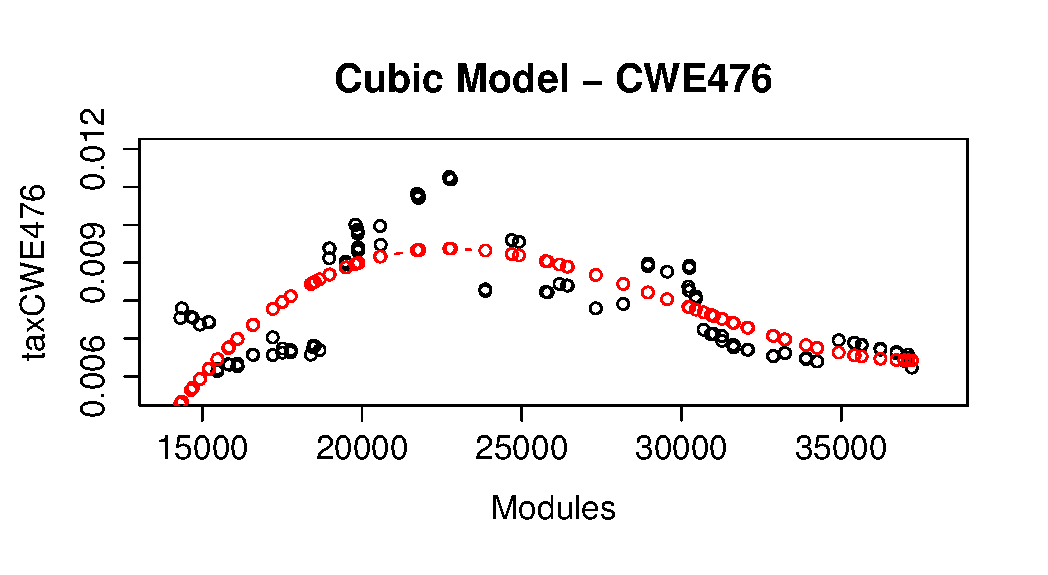
\includegraphics[width=1.0\textwidth]
      {figuras/cwe476-cubic.eps}
      \caption{Curva de predição do modelo cúbico sobre o \textit{scatterplot}
      dos dados da CWE476}
  \label{fig:cwe476-cubic}
\end{figure}


\section{Definição de modelo para CWE457 - Variável não Inicializada}

Na busca por possíveis \textit{outliers} foi contruído o gráfico
\textit{boxplot} que pode ser visto na Figura \ref{fig:cwe457-boxplot}. No caso
da CWE457 foram encontrados alguns \textit{outliers}, como pode set visto no
gráfico, alguns pontos indo além do limite do \textit{boxplot}. Foram removidos
19 pontos do conjunto de dados, não se encontrou uma justificativa plausível
para a ocorrência desses \textit{outliers}, essa decisão foi tomada apenas com o
apoio do método estatístico.

\begin{figure}[h]
  \centering
  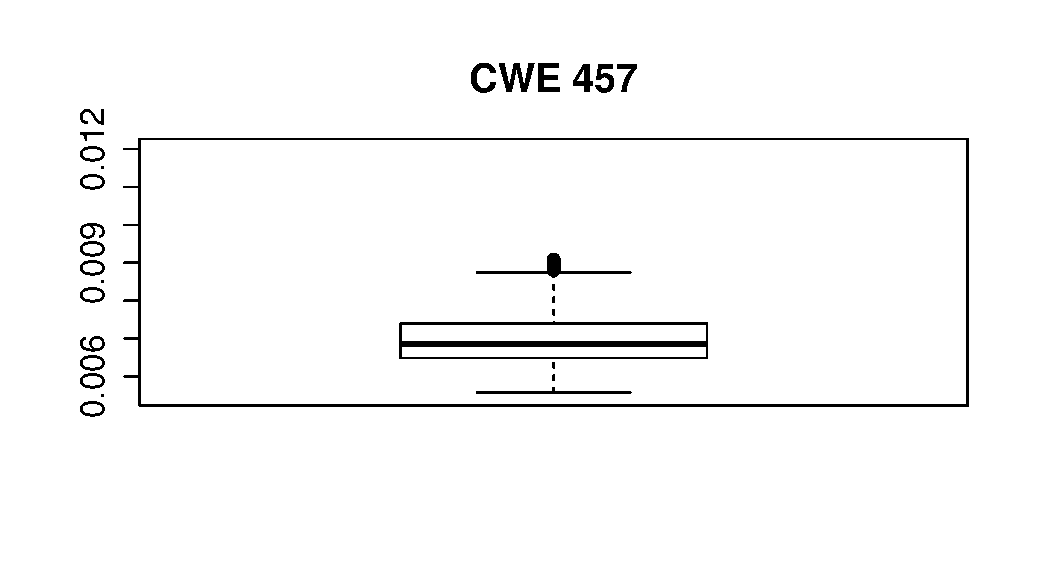
\includegraphics[width=1.0\textwidth]
      {figuras/cwe457-boxplot.eps}
      \caption{\textit{Boxplot} da taxa da CWE457 por módulo}
  \label{fig:cwe457-boxplot}
\end{figure}

Após a remoção dos \textit{outliers} identificados, foi utilizado o método
\textit{LOESS} para a geração da curva de referência. Na Figura
\ref{fig:cwe457-loess} está plotado a curva de predição do modelo gerado sobre o
\textit{scatterplot} dos dados das taxas da CWE457 por módulo. O erro residual
padrão desse modelo é 0.0003126, sendo o erro residual padrão o desvio padrão da
diferença entre o valor real e o predito.

\begin{figure}[h]
  \centering
  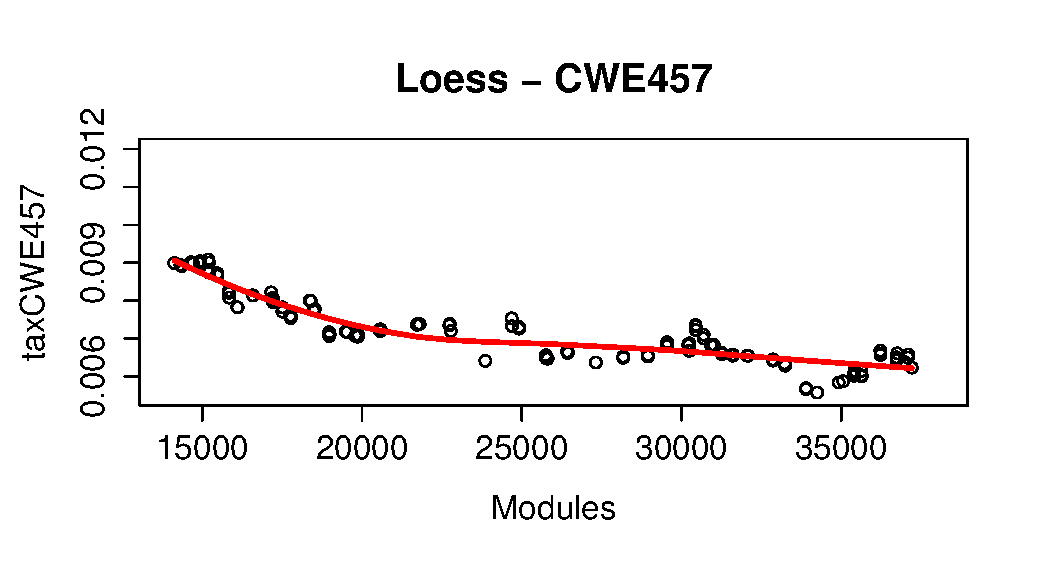
\includegraphics[width=1.0\textwidth]
      {figuras/cwe457-loess.eps}
      \caption{Curva suavizada gerada pelo método \textit{LOESS} sobre o
      conjunto de dados da taxa da CWE457 por módulo}
  \label{fig:cwe457-loess}
\end{figure}

Mais uma vez o modelo não paramétrico utilizado nos traz uma curva bastante
suave que se adapta bem aos dados trabalhados. Apesar de aparentar ser um bom
modelo, não é facilmente visível qual o grau do polinômio que melhor se
assemelha a curva gerada. Com isso, se tomou como base o trabalho realizado
sobre a CWE476, onde foram testados um modelo quadrático e um cúbico, que,
provavelmente, vão conseguir se ajustar a curva de referência, já que a mesma não
possuí muitas nuâncias.

A regressão para um polinômio quadrático do conjunto de treinamento nos deu a
seguinte equação:

\begin{align*}
 tax\_CWE457(modules) &=& (5.440273e^{-12}) * modules^{2} \\
                      &-& (3.745102ei^{-07}) * modules \\
                      &+& 0.01283622 \\
\end{align*}

Após realizada uma predição sobre o conjunto de teste, foi plotada a curva de
predição juntamento com o \textit{scatterplot} dos dados, como pode ser visto na
Figura \ref{fig:cwe457-quadratic}. O erro residual padrão para esse modelo foi
0.0003629.

\begin{figure}[h]
  \centering
  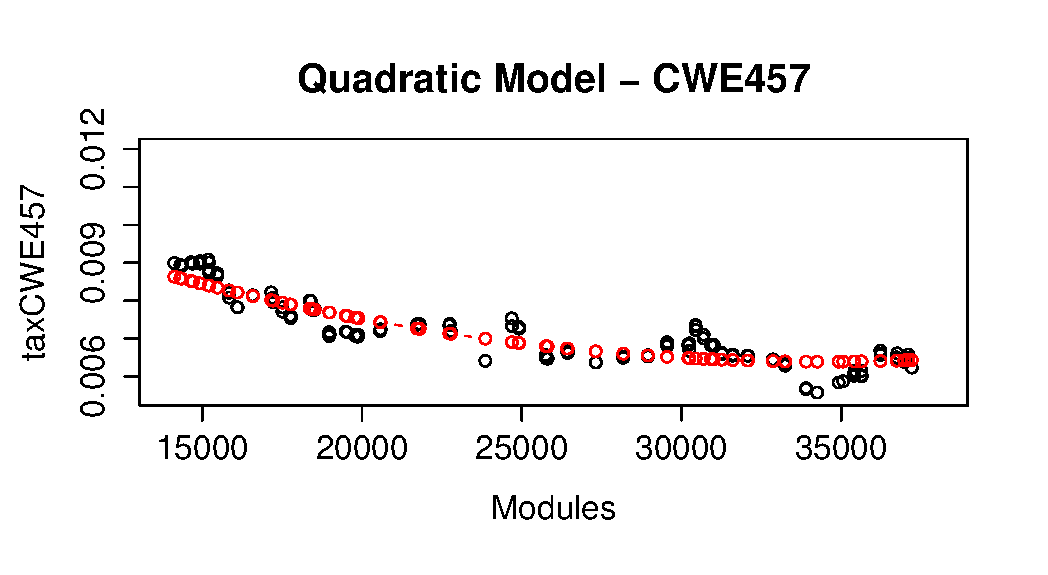
\includegraphics[width=1.0\textwidth]
      {figuras/cwe457-quadratic.eps}
      \caption{Curva de predição do modelo quadrático sobre o \textit{scatterplot}
      dos dados da CWE457}
  \label{fig:cwe457-quadratic}
\end{figure}

A regressão para um polinômio cúbico do conjunto de treinamento nos deu a
seguinte equação:

\begin{align*}
 tax\_CWE476(modules) &=& (-6.466983e^{-16}) * modules^{3} \\
                      &+& (5.603787e^{-11}) * modules^{2} \\
                      &-& (1.639652e^{-6}) * modules \\
                      &+& 0.02287291
\end{align*}

Após realizada uma predição sobre o conjunto de teste, foi plotada a curva de
predição juntamento com o \textit{scatterplot} dos dados, como pode ser visto na
Figura \ref{fig:cwe457-cubic}. O erro residual padrão para esse modelo foi
0.0003211.

\begin{figure}[h]
  \centering
  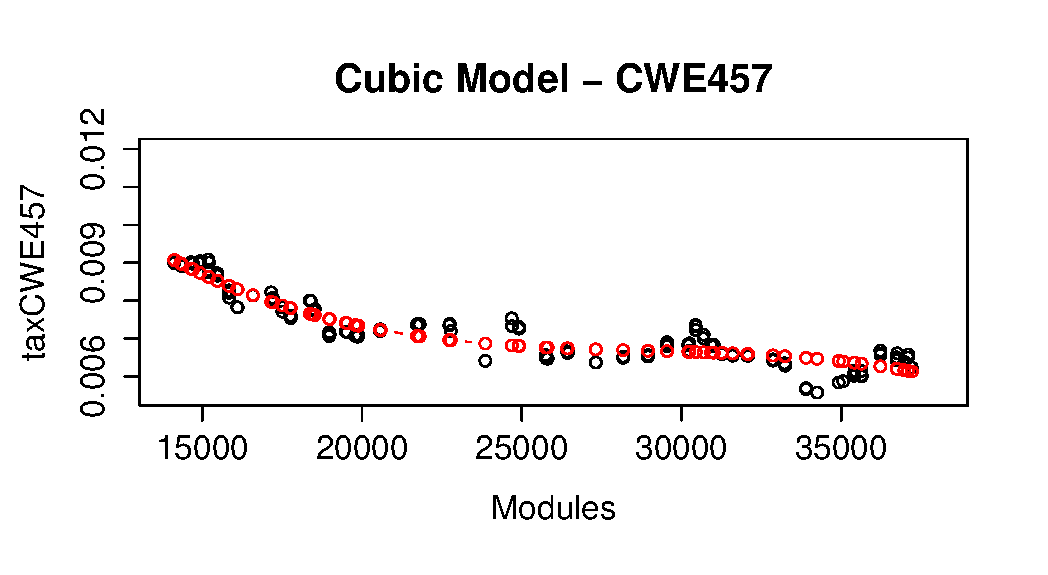
\includegraphics[width=1.0\textwidth]
      {figuras/cwe457-cubic.eps}
      \caption{Curva de predição do modelo cúbico sobre o \textit{scatterplot}
      dos dados da CWE457}
  \label{fig:cwe457-cubic}
\end{figure}

Na Tabela \ref{tab:cwe457-erros} são resumidos os erros de cada um dos modelos
definidos a partir do conjunto de dados da CWE457.

\begin{table}[h]
 \centering
 \begin{tabular}{cc}
  \hline
  \rowcolor[HTML]{EFEFEF} 
  {Modelo} & {Erro residual padrão} \\ \hline
  {LOESS}  & 0.0003126                  \\ \hline
  Quadrático   & 0.0003629                  \\ \hline
  Cúbico       & 0.0003211                \\ \hline 
 \end{tabular}
 \caption{Resumo do erro residual padrão dos modelos contruídos para as taxas da
 CWE457}
 \label{tab:cwe457-erros}
\end{table}




\section{Comparação e Escolha dos Modelos}\label{comparacaomodelos}

Na Seção \ref{definicaomodelos} foram definidos dois modelos para cada uma das
métricas de ameaças de vulnerabilidade de código fonte, nesta Seção esses
modelos serão comparados, baseado no erro na predição do modelo e no método
\textit{K-fold} de validação cruzada, e então serão selecionados os melhores
modelos. Nesta Seção foi feita uma comparação e escolha entre os modelos
desenvolvidos, podendo existir modelos melhores para cada uma das métricas.

Pensou-se em realizar uma Análise de Variância (\textit{ANOVA}) para tentar
auxiliar na comparação entre os modelos, mas não foi possível já que o conjunto
de dados das taxas das CWE476 e CWE457 por módulo não respeitam as suposições a
cerca da \textit{ANOVA} apresentadas na Seção \ref{valmodels}, como pode ser visto
durante a análise exploratória dos dados nas seções \ref{eda:cwe457} e
\ref{eda:cwe476}.

Observa-se que quanto maior o grau do polinômio melhor serão os resultados
obtidos, entretanto, o objetivo deste trabalho é encontrar um modelo simples,
que não seja muito custoso, onde o mesmo possa ser inserido sem muitos problemas
no ciclo de desenvolvimento de software. Devido a isso foram selecionados
modelos de baixo grau, onde a complexidade das funções obtidas são bem menores.

Tendo isso em vista, foram analisados e comparados os modelos de cada uma das
métricas separadamente, como pode ser visto a seguir.

\subsection{CWE476 - Referência de Ponteiros Nulos}\label{comparacaocwe476}

Para iniciar a comparação foram confrontados todos os modelos em um único
gráfico (Figura \ref{fig:cwe476-all-models}), que pode nos dar uma visão geral de
como os modelos estão realizando as suas respectivas predições.

\begin{figure}[h]
  \centering
  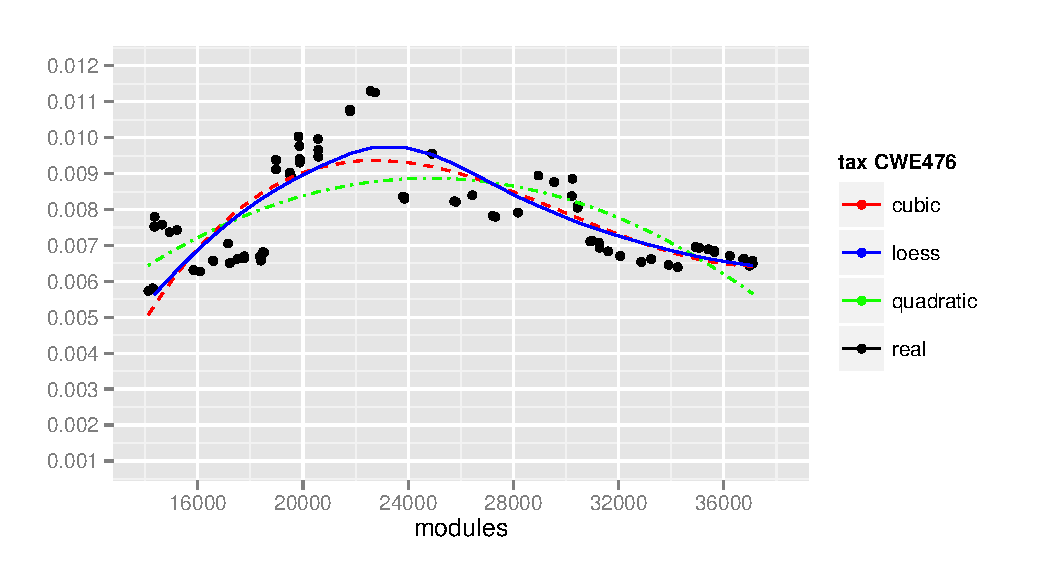
\includegraphics[width=1.0\textwidth]
      {figuras/cwe476-all-models.eps}
      \caption{Curva de predição de todos os modelos sobre o \textit{scatterplot}
      dos dados da CWE476}
  \label{fig:cwe476-all-models}
\end{figure}

A Figura \ref{fig:cwe476-all-models} nos mostra de maneira visual que o modelo
cúbico gerado é o que melhor se aproxima da curva de predição do modelo de
referência (modelo \textit{LOESS}, não paramétrico), principalmente no que diz
respeito a extrapolação, tanto para dados menores ou maiores ao intervalo de
dados trabalhados nesta pesquisa. Essa extrapolação é importante para que seja
possível a predição da métrica, por exemplo, para projetos com mais de 40.000 ou
com menos de 14.000 módulos. O modelo cúbico acompanha de maneira mais adequada
nos limites do gráfico o modelo de referência, e o modelo quadrático tende a se
distanciar nesses locais.

Saindo da parte visual e partindo para o erro residual padrão, sendo o erro
residual padrão o desvio padrão da diferença entre o valor real e o predito,
gerado por cada um dos modelos, que podem ser vistos na Tabela
\ref{tab:cwe476-erros}. Percebe-se que o erro referente ao modelo cúbico se
aproxima bastante ao nosso modelo de referência (\textit{LOESS}). O erro
associado ao modelo quadrático é aproximadamente 20,00\% maior do que o do
modelo de referência, já o cúbico é aproximandamente 4,43\% maior. Logo, o erro
entre os modelos quadrático e cúbico é de aproximadamente 15\%, sendo o cúbico
mais próximo do desejável.

\begin{table}[h]
 \centering
 \begin{tabular}{cc}
  \hline
  \rowcolor[HTML]{EFEFEF} 
  {Modelo} & {Erro residual padrão} \\ \hline
  {LOESS}  & 0.0008044                  \\ \hline
  Quadrático   & 0.0009653                  \\ \hline
  Cúbico       & 0.0008400                \\ \hline 
 \end{tabular}
 \caption{Resumo do erro residual padrão dos modelos contruídos para as taxas da
 CWE476}
 \label{tab:cwe476-erros}
\end{table}

Para finalizar a comparação entre os modelos foi realizado uma validação cruzada
utilizando o método \textit{K-fold} para analisar a performance de ambos o
modelos em um conjunto de dados cujo qual não foi treinado, ou seja, contra
dados que o mesmo deveria predizer em uma situação real. Nesta pesquisa foi
utilizado um \textit{K} = 10, já que segundo \citeonline{kohavi:1995} uma
validação cruzada \textit{ten-fold} pode ser mais eficiente até que uma
validação cruzada \textit{leave-one-out}, mais detalhes sobre o assunto pode ser
visto na Seção \ref{valmodels}. Os gráficos apresentados nas figuras
\ref{fig:cwe476-k-fold-quadratic} e \ref{fig:cwe476-k-fold-cubic} nos mostra um
resumo do método aplicado.

\begin{figure}[h]
  \centering
  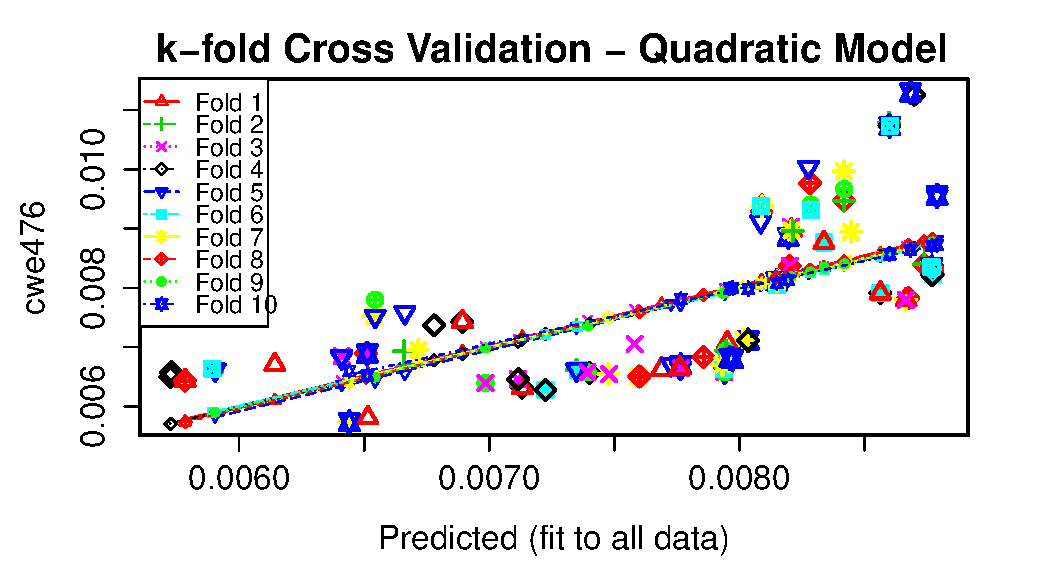
\includegraphics[width=1.0\textwidth]
      {figuras/cwe476-k-fold-quadratic.eps}
      \caption{Validação cruzada \textit{Ten-fold} utilizando o modelo
      quadrático da taxa da CWE476}
  \label{fig:cwe476-k-fold-quadratic}
\end{figure}

\begin{figure}[h]
  \centering
  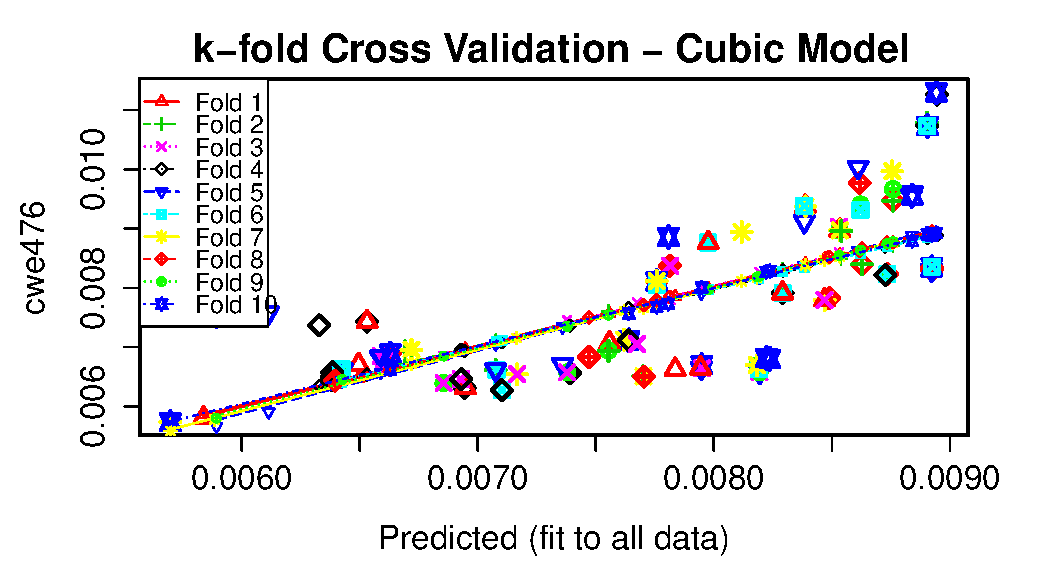
\includegraphics[width=1.0\textwidth]
      {figuras/cwe476-k-fold-cubic.eps}
      \caption{Validação cruzada \textit{Ten-fold} utilizando o modelo
      cúbico da taxa da CWE476}
  \label{fig:cwe476-k-fold-cubic}
\end{figure}

O gráficos apresentados possuem no eixo X os valores preditos pelo modelo em
questão e no eixo Y o valor real. As retas traçadas representam o que seria o
ideal, ou seja, o valor predito igual ao valor real, e cada um dos diferentes
pontos apresentam o que foi gerado pelo modelo em cada um dos \textit{folds}.
Pode-se ver que em ambos os gráficos vários pontos ficaram distantes da reta,
mostrando que existe um erro associado a predição. Na Tabela
\ref{tab:cwe476-emq} são apresentados os erros médios quadráticos de cada um dos
modelos aqui avaliados, a definição de erro médio quadrático pode ser encontrada
na Seção \ref{valmodels}.

\begin{table}[h]
 \centering
 \begin{tabular}{cc}
  \hline
  \rowcolor[HTML]{EFEFEF} 
  {Modelo} & {Erro médio quadrático} \\ \hline
  Quadrático   & 0.000000958                  \\ \hline
  Cúbico       & 0.000000862                 \\ \hline
 \end{tabular}
 \caption{Resumo do erro residual quadrático dos modelos contruídos para as taxas da
 CWE476 através da validação cruzada.}
 \label{tab:cwe476-erros}
\end{table}

Pode-se ver que mais uma vez o modelo cúbico se sobressaiu ao modelo quadrático,
sendo o erro médio quadrático associado ao modelo quadrático aproximadamente
11,14\% maior do que o modelo cúbico em situações reais de análise.

Levando em consideração todos os aspectos trabalhados na comparação dos dois
modelos, o modelo cúbico se apresentou como um melhor modelo para o
acompanhamento, monitoramento e predição da taxa da ameaça de vulnerabilidade de
código fonte relacionada a referência de ponteiros nulos.

\subsection{CWE457 - Variável não Inicializada}

Para uma melhor visualização dos modelos construídos foi contruído um gráfico
contendo a curva de predição de todos eles sobre o \textit{scatterplot} dos
dados. Esse gráfico pode ser visto na Figura \ref{fig:cwe457-all-models}.

\begin{figure}[h]
  \centering
  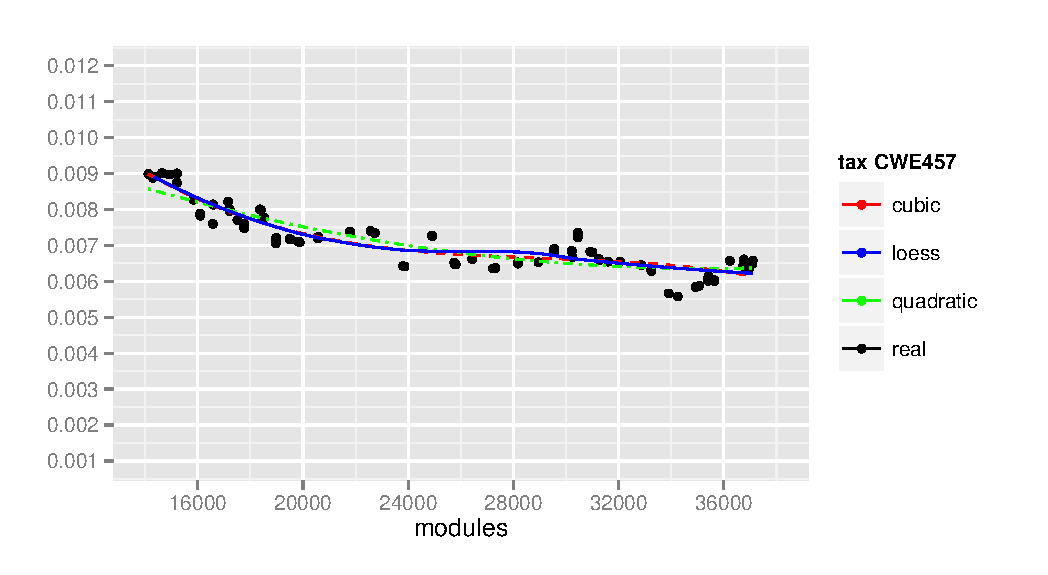
\includegraphics[width=1.0\textwidth]
      {figuras/cwe457-all-models.eps}
      \caption{Curva de predição de todos os modelos sobre o \textit{scatterplot}
      dos dados da CWE457}
  \label{fig:cwe457-all-models}
\end{figure}

Todos os modelos apresentados na Figura \ref{fig:cwe457-all-models} ficaram bem
próximos uns dos outros, diferente do ocorrido com os modelos referentes a
CWE476. Entretanto, o modelo cúbico continua mais próximo do modelo de
referência (\textit{LOESS}) nos limites mínimo e máximo em relação ao modelo
quadrático, sendo similar a comparação dos modelos na Seção
\ref{comparacaocwe476}, o que favorece predições de valores fora do intervalo de
valores trabalhados neste estudo.

Visualmente também pode-se ver que provavelmente o erro residual desses modelos
são bem menores do que os análisados na Seção \ref{comparacaocwe476}. Na Tabela
\ref{tab:cwe457-erros} são apresentados os erros residuais padrão de cada um dos
modelos, mais sobre erro residual padrão pode ser visto na Seção \ref{valmodels}.

\begin{table}[h]
 \centering
 \begin{tabular}{cc}
  \hline
  \rowcolor[HTML]{EFEFEF} 
  {Modelo} & {Erro residual padrão} \\ \hline
  {LOESS}  & 0.0003287                  \\ \hline
  Quadrático   & 0.0003674                  \\ \hline
  Cúbico       & 0.0003388                 \\ \hline
 \end{tabular}
 \caption{Resumo do erro residual padrão dos modelos contruídos para as taxas da
 CWE457}
 \label{tab:cwe457-erros}
\end{table}

Como foi dito anteriormente, os erros residuais padrão dos modelos apresentados
possuíram valores baixos e com uma pequena diferença entre os mesmos, apesar do
modelo cúbico estar mais próximo do modelo de referência. O modelo quadrático
teve um erro 11,77\% maior do que o modelo de referência e o modelo cúbico
3,07\% maior, logo, o modelo quadrático teve um erro 8,44\% maior do que o
modelo cúbico. Mais uma vez o modelo cúbico apresentado um erro menor do que o
modelo quadrático.

Para verificar o desempenho de cada um dos modelos foi feita uma validação
cruzada \textit{K-fold}. Assim como na Seção \ref{comparacaocwe476}, foi
utilizado um \textit{K} = 10. Os gráficos apresentados nas figuras
\ref{fig:cwe457-k-fold-quadratic} e \ref{fig:cwe457-k-fold-cubic} nos mostra um
resumo dos testes realizados.

\begin{figure}[h]
  \centering
  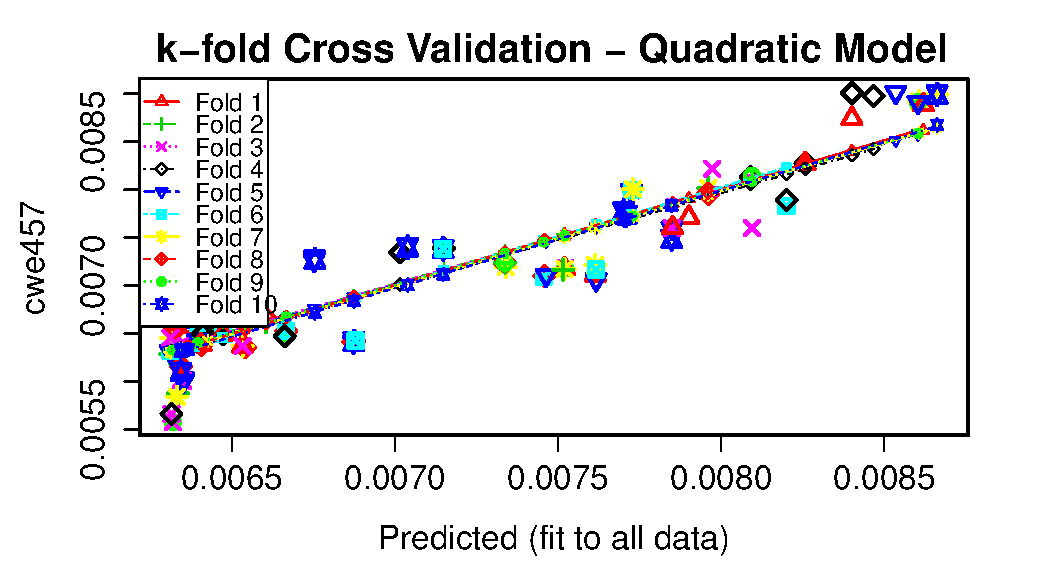
\includegraphics[width=1.0\textwidth]
      {figuras/cwe457-k-fold-quadratic.eps}
      \caption{Validação cruzada \textit{Ten-fold} utilizando o modelo
      quadrático da taxa da CWE457}
  \label{fig:cwe457-k-fold-quadratic}
\end{figure}

\begin{figure}[h]
  \centering
  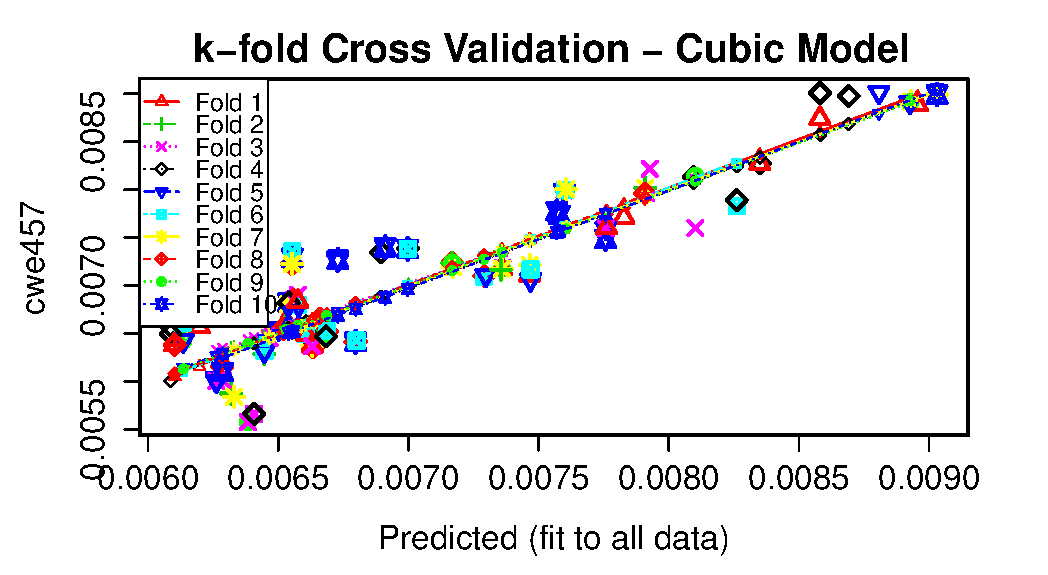
\includegraphics[width=1.0\textwidth]
      {figuras/cwe457-k-fold-cubic.eps}
      \caption{Validação cruzada \textit{Ten-fold} utilizando o modelo
      cúbico da taxa da CWE457}
  \label{fig:cwe457-k-fold-cubic}
\end{figure}

Definições acerca do método \textit{K-fold} de validação cruzada podem ser
encontradas na Seção \ref{k-fold}. A Tabela \ref{tab:cwe457-emq} apresenta os
erros médios quadráticos obtidos através da validação cruzada.

\begin{table}[h]
 \centering
 \begin{tabular}{cc}
  \hline
  \rowcolor[HTML]{EFEFEF} 
  {Modelo} & {Erro médio quadrático} \\ \hline
  Quadrático   & 0.000000137 \\ \hline
  Cúbico       & 0.000000112 \\ \hline
 \end{tabular}
 \caption{Resumo do erro residual quadrático dos modelos contruídos para as taxas da
 CWE457 através da validação cruzada.}
 \label{tab:cwe457-emq}
\end{table}

O erro médio quadrático referente ao modelo cúbico se apresentou 22,32\% menor
do que do modelo quadrático. Apesar da diferença percentual aparentar ser
grande, numericamente pode não ser tão significativo, essa diferença percentual
é devido ao erro ser bem pequeno, onde qualquer pequena diferença representa um
grande percentual.

Apesar do modelo cúbico se apresentar mais vantajoso durante a comparação
realizada, o modelo quadrático também se mostrou como uma boa solução para o
acompanhamento, monitoramento e predição desta métrica de ameaça de
vulnerabilidade de código fonte, já que a diferença no geral foi pequena. Logo,
a seleção de qualquer um dos modelos seria uma boa escolha, o modelo quadrático
tendo uma complexidade menor, e o modelo cúbico acompanhando de maneira
mais adequado o modelo de referência nos limites apresentados, o que favorece a
extrapolação dos valores. Tendo em vista que este trabalho visa principalmente
a predição dos valores das métricas em questão, o modelo cúbico foi selecionado
devido a maior aderência ao modelo de referência escolhido.


\section{Consolidação dos Resultados}

Com o que se diz respeito a hipótese \textit{H4}, foram definidos dois modelos e
selecionado um para cada uma das métricas de ameaças de vulnerabilidade de
código fonte. Essa hipótese também não foi negada, já que como foi apresentado
na comparação entre os modelos (Seção \ref{comparacaomodelos}), os mesmos se
apresentaram bem diante de situações reais de análise, logo, atingindo o
objetivo de acompanhar, monitorar e predizer valores das métricas de maneira
satisfatória. Entretanto, como foi explicado nas seções \ref{definicaomodelos} e
\ref{comparacaomodelos}, quanto maior o grau do polinômio melhor ele se adaptará
aos dados e menor será o erro associado ao conjunto de treinamento. A estratégia
de utilizar um modelo não paramétrico foi justamente para evitar esse
\textit{overfitting} dos dados, além disso, tentou-se manter o foco em modelos
polinômiais de baixa complexidade, que julgou-se mais fácil de serem
incorporados no dia-a-dia do desenvolvimento de software.

Após a realização da comparação e seleção dos modelos para cada uma das métricas
de ameças de vulnerabilidade de código fonte, chegou-se a seguinte função para
cada uma das métricas trabalhadas:

\begin{align*}
 tax\_CWE476(modules) &=& (1.911224e^{-15}) * modules^{3} \\
                      &-& (1.72028e^{-10}) * modules^{2} \\
                      &+& (4.857479e^{-6}) * modules \\
                      &-& 0.03460173
\end{align*}

\begin{align*}
 tax\_CWE476(modules) &=& (-6.466983e^{-16}) * modules^{3} \\
                      &+& (5.603787e^{-11}) * modules^{2} \\
                      &-& (1.639652e^{-6}) * modules \\
                      &+& 0.02287291
\end{align*}

Lembrando que as fórmulas matemáticas apresentadas acima representam os modelos
desenvolvidos na seção \ref{definicaomodelos}, ambos sendo desenvovlidos a
partir de uma regressão polinomial de terceiro grau das métricas obtidas a
partir do código fonte do projeto \textit{Linux Kernel}.

Para apresentar os modelos definidos foram elaboradas as Tabelas
\ref{tab:cwe476} e \ref{tab:cwe457} que apresentam os valores das referidas
métricas em alguns determinados pontos já conhecidos, sendo eles a primeira
versão, a última versão e a versão com o valor da métrica mais alto, e ao final
um novo ponto predito pelo modelo construído.

\begin{table}[h]
\centering
\begin{tabular}{ccc}
\hline
\rowcolor[HTML]{EFEFEF} 
{Version}  & {tax\_CWE476} & {Modules} \\ \hline
linux-v2.6.11  & 0.005735325       & 14123         \\ \hline
linux-v2.6.39  & 0.008927095       & 30245         \\ \hline
linux-v3.9-rc8 & 0.006460368       & 33899         \\ \hline
X              & 0.008715918       & 43787         \\ \hline
\end{tabular}
\caption{Alguns valores da taxa da CWE476 mais predição realizada.}
\label{tab:cwe476}
\end{table}

\begin{table}[h]
\centering
\begin{tabular}{ccc}
\hline
\rowcolor[HTML]{EFEFEF} 
{Version}   & {tax\_CWE457} & {Modules} \\ \hline
linux-v2.6.11   & 0.008992424       & 14123         \\ \hline
linux-v3.16-rc3 & 0.006577706       & 37095         \\ \hline
linux-v3.9-rc8  & 0.005663884       & 33899         \\ \hline
X               & 0.004226781       & 43787         \\ \hline
\end{tabular}
\caption{Alguns valores da taxa da CWE457 mais predição realizada.}
\label{tab:cwe457}
\end{table}

Para selecionar o ponto que foi predito foi feita a média da diferença entre os
módulos dos outros pontos selecionados, que coincidentemente foi o mesmo para
ambas as métricas, apesar dos pontos conhecidos selecionados serem diferentes.
Como pode-se ver na Tabela \ref{tab:cwe476}, a métrica relacionada a taxa da
CWE476 teve um pico na versão 2.6.39 e depois começou a diminuir, mas a partir do
momento que o número de módulos voltar a crescer ela tende a crescer novamente,
e em determinado ponto deve atingir um novo pico e voltar a diminuir o seu
valor. Com a métrica relacionado a taxa da CWE457 já é diferente, pelo o que foi
apresentado na Tabela \ref{tab:cwe457} a métrica tende a diminuir sempre com o
decorrer do aumento do número de módulos.

Para exemplificar o uso dos modelos desenvolvidos serão apresentados na Seção
\ref{exemplosdeuso} alguns exemplos de uso do mesmo com alguns dos projetos de
software trabalhados na primeira etapa da pesquisa. Lembrando, que esses modelos
baseados no projeto \textit{Linux Kernel} visam servir de referência para outros
projetos.




\section{Exemplos de Uso}\label{exemplosdeuso}

Para dar alguns exemplos palpáveis do uso dos modelos desenvolvidos em um
projeto de softwares livre foram realizadas predições das métricas das taxas das
CWE476 e CWE457 em projetos trabalhados na primeira etapa do projeto. Foram
selecionados 5 projetos de software, cujo quais são:

\begin{itemize}
 \item Bash
 \item OpenSSH
 \item OpenSSL
 \item Python2.7
 \item Ruby-2.1
\end{itemize}

Para apresentar a utilização dos modelos, foram preditos os valores das métricas
para esses projetos, sem necessariamente realizar uma análise estática sobre os
mesmos. Dessa forma, na Tabela \ref{tab:exemplos} são apresentadas os valores
das métricas em questão esperados para cada um dos projetos, baseado no modelo de
referência construído a partir do projeto \textit{Linux Kernel}.

\begin{table}[h]
 \centering
 \begin{tabular}{ccll}
  \hline
  \rowcolor[HTML]{EFEFEF} 
  Projeto de Software & Módulos &
  \multicolumn{1}{c}{\cellcolor[HTML]{EFEFEF}tax\_CWE476} &
  \multicolumn{1}{c}{\cellcolor[HTML]{EFEFEF}tax\_CWE457} \\ \hline
  Bash                & 369     & -0.02738566
  & 0.02227548                                              \\ \hline
  OpenSSH             & 364     & -0.02740602
  & 0.02228347                                              \\ \hline
  OpenSSL             & 1164    & -0.02423955
  & 0.02103926                                              \\ \hline
  Python2.7           & 808     & -0.02562603
  & 0.02158432                                              \\ \hline
  Ruby-2.1            & 547     & -0.02666550
  & 0.02199268                                             \\ \hline
 \end{tabular}
 \caption{Predição de métricas em projetos de software livre com menor número
 de módulos.}
 \label{tab:exemplos}
\end{table}


Como apresentado na Tabela \ref{tab:exemplos} a predição para valores da
métricas relacionada a taxa da CWE457 parece algo razoável e dentro do esperado,
entretanto, não se pode dizer o mesmo dos valores da métrica referente a taxa da
CWE476. Na elaboração desses exemplos de uso percebeu-se uma limitação do
modelo de predição desenvolvido para a métrica relacionada a referência de
ponteiros nulos (CWE476), onde o modelo não se apresentou de maneira adequada
para a predição da métrica para projetos com quantidade de módulos muito menor
do que foi contruído (a versão do \textit{Linux Kernel} com menor número de
módulos possui 14123). Percebeu-se que o modelo desenvolvido apresenta valores
negativos para a métrica em questão quando o número de módulos é menor do que
10105, sendo que a métrica não aceita valores menores do que zero. Esse
comportamento é justificado quando se observa o gráfico (Figura
\ref{fig:cwe476-cubic}) que apresenta a linha de predição do modelo, pode-se ver
que quanto menor o número de módulos a partir de 14234 a tendência do modelo é
predizer valores menores, com uma taxa de queda do valor da métrica bastante
acentuada. Logo, o modelo desenvolvido para a métrica referente a taxa da CWE476
não se aplica para números de módulos pequenos, diferente da CWE457,
provavelmete, conseguindo predizer valores para a métrica para projetos de
software maiores do que 10100 módulos.

Tendo em vista a limitação do modelo desenvolvido relacionado a métrica de taxa
de CWE476 por módulo identificada para projetos com números de módulos menores
do que os que o mesmo foi construído, resolveu-se testar os modelos com projetos
de softwares livre maiores com o que se diz respeito ao número de módulos, a fim
de validar a utilização dos modelos para esse tipo de projeto. Para isso foram
selecionados dois novos projetos de software livre, sendo eles o
\textit{FreeBSD} e o \textit{Android}, ambos inclusive tendo em comum com o
\textit{Linux Kernel} o desenvolvimento de um núcleo de um sistema operacional.
Foi desenvolvida a Tabela \ref{tab:exemplos2}, similar a anterior (Tabela
\ref{tab:exemplos}), para tentarmos verificar o uso dos modelos de predição em
projetos de software livre com uma maior quantidade de números de módulos.

\begin{table}[h]
 \centering
 \begin{tabular}{ccll}
  \hline
  \rowcolor[HTML]{EFEFEF} 
  Projeto de Software & Módulos &
  \multicolumn{1}{c}{\cellcolor[HTML]{EFEFEF}tax\_CWE476} &
  \multicolumn{1}{c}{\cellcolor[HTML]{EFEFEF}tax\_CWE457} \\ \hline
  FreeBSD             & 33203   & 0.0069897180
  & 0.0065379640                                           \\ \hline
  Android             & 49431   & 0.0160103100
  & 0.0006387576                                          \\ \hline
 \end{tabular}
 \caption{Predição de métricas em projetos de software livre com maior número
 de módulos.}
 \label{tab:exemplos2}
\end{table}

Pode-ser ver na Tabela \ref{tab:exemplos2} que ambos os modelos se comportaram
de maneira adequada e dentro do esperado, com valores de métricas aceitáveis,
para projetos de software com a quantidade de número de módulos igual ou maior
ao que os mesmos foram construídos baseado no projeto \textit{Linux Kernel}. O
projeto \textit{FreeBSD} se apresenta em um estágio similar ao \textit{Linux
Kernel}, onde os mesmos possuem um número de módulos e valores de ambas as
métricas similares quando se comparando os dados das Tabelas
\ref{tab:exemplos2}, \ref{tab:cwe476} e \ref{tab:cwe457}, levando em
consideração a última versão do \textit{Linux Kernel}. Já o projeto
\textit{Android} se apresenta com uma quantidade de módulos muito maior do que
os outros dois projetos mencionados, a primeira vista aparenta que talvez o
projeto esteja em um estágio mais imaturo e necessite de uma refatoração para
atingir o patamar dos outros, entretanto, essa diferença é grande devido ao
repositório do projeto \textit{Android} não conter apenas o núcleo do seu
sistema operacional, mas sim vários outras coisas como ABI (\textit{Application
Binary Interface}), \textit{frameworks}, suas próprias ferramentas de
desenvolvimento entre outras coisas. 

Logo, pode-se sinalizar nessa primeira análise que o modelo de predição
referente a variáveis não inicializadas por módulo (CWE457) apresenta valores
adequados de predição tanto para projetos com um menor número de módulos quanto
para maiores, já o modelo de predição referente a referência a ponteiros nulos
por módulo (CWE476) traz valores de predição aceitáveis para a métrica apenas
para projetos que possuem mais de 10100 módulos. 

Portanto, com os modelos desenvolvidos foi possível realizar a predição das
métricas em questão para projetos do mesmo porte da referência selecionada
(\textit{Linux Kernel}), sendo esses a principal contribuição desta pesquisa. Os
resultados obtidos foram satisfatórios tendo em vista que foi possível realizar
as predições das métricas de ameaças de vulnerabilidade de código fonte
propostas, sendo esse o objetivo maior deste trabalho.

